\chapter{Compiler} \label{sec:compiler}

In this section, we introduce the compiler framework---\name---that targets Plasticine
architecture from high-level programs described in the Spatial language. 

In the following sections, \Cref{sec:control} describes conversion from an imperative paradigm with
a nested control hierarchy to the distributed streaming dataflow execution.
\Cref{sec:resalloc} details program-partitioning passes that decompose program over distributed resources.
\Cref{sec:opt} enumerates several optimizations in \name, and \Cref{sec:par} discuss about PaR and
heuristic generation.

\section{\name Compiler Overview} \label{sec:compileroverview}

In this section, we introduce the compiler framework---\name---that targets Plasticine
architecture from high-level programs described in the Spatial language. 
There are two challenges to map Spatial applications to Plasticine. 

First, unlike an FPGA, Plasticine cannot map arbitrary RTL functionality.
In the Spatial abstraction, the execution order of the program is organized by a control hierarchy, where
each level of the controller schedules the execution of the next level controllers.
When mapping the example in \Cref{fig:spatialegpar} onto an FPGA, the outer controller \emph{A}
sends an enable signal to each child controller, which signals back the parent controller when
completed. If the user chooses to sequentially execute the outer loop \emph{A}, the parent
controller enables the child controllers one at a time; if the user chooses to metapipeline
(coarse-grain pipeline) the outer loop \emph{A}, the outer controllers enables multiple child controllers in a pipelined fashion.

\begin{figure*}
\centering
  \centering
\includegraphics[width=0.8\textwidth]{figs/centralctrl.pdf}
\caption{
  (a) A na\"ive mapping strategy to map the control hierarchy onto Plasticine.
  All units are distributed across an on-chip network that can introduce unpredictable latency.
  The number on the edges indicates event order.
  Here we show a scenario where read requests from \emph{C} do not observe the write requests from
  \emph{B} that occur earlier in the program order due to network latency between \emph{B} and
  \emph{mem}.
  (b) Distributed controllers in \name. Each innermost controller makes a copy of all enclosing controllers. The signals from these controllers are used to generate synchronization between distributed compute units. To address the problem in (a), the memory also needs to provide a write acknowledgment per write request for synchronization.
}
\label{fig:centralctrl}
\end{figure*}

To achieve the same execution schedule on Plasticine in a na\"ive approach, 
we can map each controller in the hierarchy into a PU, sending control signals to schedule the next level controllers distributed in other PUs, as shown in \Cref{fig:centralctrl} (a).
This strategy suffers from the expensive network round-trip delays between the parent and child controllers.
To be scalable at a high clock frequency, Plasticine networks are pipelined at each switch,
introducing multiple cycles of network delay across PUs on the control path.
Therefore, the multi-cycle handshaking signal between the parent and the child can introduce significant pipeline bubbles
that undermines performance.
Additionally, this scheme creates a communication hotspot around the parent controller \emph{A} as
loop \emph{A} gets unrolled, which is devastating for a CGRA
like Plasticine that has much less routing resource than an FPGA.
Furthermore, synchronizing the compute only is insufficient to ensure memory effects are observed by
the remotely distributed accessors, as shown in \Cref{fig:centralctrl} (a).

To address this challenge, we want to eliminate centralized outer controllers.
At high-level, \name performs loop divisions (discussed later in ~\Cref{sec:loopdiv}) on each outer controller, such that
all innermost controllers are perfectly nested, as shown in \Cref{fig:centralctrl} (b).
\name then allocates synchronization tokens across the distributed innermost controllers.
All innermost controllers have their own copies of the outer controllers, which are used to
generate the control tokens.
These control tokens ensure the execution order of the inner controllers is the same as if they are
scheduled by a centralized outer controller. Instead of synchronizing all inner controllers under an outer controller, \name only synchronizes the ones accessing the same memory, such as \emph{B} and
\emph{C} in \Cref{fig:spatialegpar}. This limits the synchronization among a small set of
distributed nodes without impacting the result, 
making our design much more scalable.

The second challenge in this mapping process is that controllers in the spatial hierarchy
can consume an arbitrary amount of compute and memory resources, exceeding the capacity of individual
PUs. For instance, a user might write a memory multiple times throughout the program with writers mapped to different PUs. The physical scratchpad, however, only has a single write
port. 
\name generates control tokens among the distributed writers to time-share the write port and enforce the ordering between writers.
With resource virtualization, \name composes or time-share the physical resources when software usage exceeding the hardware limit.

\begin{figure*}
\centering
\includegraphics[width=1\textwidth]{figs/sarastack.pdf}
\caption[\name Compiler Flow]{\name Compiler Flow}
\label{fig:flow}
\end{figure*}
 
In the following sections, we describe a systematic approach to compile applications described in an
imperative front-end language to a purely declarative and distributed dataflow graph that can
run on Plasticine. \Cref{fig:flow} shows \name's compilation flow.

\Cref{sec:control} expands on the \term{imperative to streaming transformation} that
addresses the first challenge.
\name allocates distributed on-chip resources to execute the program in spatially parallelized and
pipelined fashion with appropriate synchronizations.
A virtual unit (VU) is our intermediate representation that captures the computation mapped
within the boundary of a physical unit (PU), such as a PCU and PMU.
Each VU can contain multiple contexts if their aggregated resource usage can fit in a PU.
The hardware can limit the maximum number of contexts a PU can support and has resources that cannot be split across contexts.
Most importantly, \name needs to ensure messages across VUs, which are mapped across the global network, tolerate an arbitrary amount of network latencies; messages within a single VU across contexts takes only a single cycle.
The transformation phase generates a virtual unit dataflow graph (VUDFG) with appropriate
synchronizations, such that a streaming pipelined execution over distributed on-chip resources produces the same result as a
parallelized program executed in time.
At the end of the allocation phase, a virtual unit can consume as many resources as the program
requires. 

\name further virtualizes resource allocation and hides the underlying resource constraints on
this hierarchical architecture from the programmers.
\Cref{sec:resalloc} dives into the \term{resource allocation} phase, where \name assigns each VU to a
PU that processes the required resources. If no PU can fit a VU, \name partitions the
VU into multiple VUs to resolve the constraint violation. If there is insufficient PU or the VU cannot be partitioned, the mapping process fails with appropriate hints to the programmer for the
limiting resources.

Throughout the first two phases, \name introduces various \term{optimizations} that either reduce the
the resource cost of the VUDFG, or alleviates potential performance bottleneck in the streaming
pipeline.
After all VU fits in at least one type of PU, \name performs a global optimization that merges small VUs into a larger VU to reduce resource fragmentations.
\Cref{sec:opt} enumerates the optimizations \name performs.

The output of the resource allocation phase is a VUDFG with a tagged PU type for each VU.
It is up to the
\term{placement and routing (PaR)} phase to determine where the VU will be finally placed.
Right before PaR, \name performs static analysis on the traffic pattern and generate heuristic guild
for the placer to reduce routing congestion.
\Cref{sec:par} details the PaR algorithm and heuristic-guild generated by \name.


\section{Imperative to Streaming Transformation}
\label{sec:control}

%In a na\"ive approach, we can map each controller in the hierarchy into a VB (\Cref{fig:centralctrl}).
%This strategy suffers from expensive network round-trip delays between the parent and child controllers.
%If the parent controller is an unrolled loop, the parent needs to synchronize with all child controllers, which creates an undesired communication hot spot.
%\Cref{fig:centralctrl}(a) shows an example where synchronization {\em just} between parent and child controllers can produce an incorrect result due to unpredictable network latency.

%The alternative approach explores a different way to execute the expected control schedule correctly. 
%The minimum required synchronization to produce the correct result is to ensure that the computations access the intermediate results in a consistent matter as if the control schedule is strictly enforced. 
%This can be achieved via p2p synchronizations \emph{only} between computations that access a particular shared memory.
%The execution order of computations that access different memories does not need to be enforced, as they do not impact the program outcome.
%Therefore, as long as the computation is executed with the expected number of iterations and the memories are updated consistently, there is no need for any extra synchronization.
%Next, we walk through how \name{} achieves this in more concrete detail.

\subsection{Loop Division (Ready)}
Between the front-end and the back-end abstractions of \name, an obvious gap is that 
the imperative front-end language can contain arbitrarily nested control hierarchy, whereas
the hardware compute engine can only execute operations that are control-free.
To address this issue, we introduce a new type of loop transformation---loop division---for streaming reconfigurable
accelerators.
Similar to loop fission, loop division breaks a single loop into multiple loops.
The difference is that loop fission generates a sequence of sequentially executed loops, whereas
loop division generates loops executing \emph{concurrently}.
Additionally, loop fission materializes the intermediate results across fissioned loops into arrays,
while loop division use queue to communicate across loops.
Each loop generated from loop division can only execute if all of their input queues are not empty.
\Cref{fig:loopexp1} gives an example of a loop fusion vs. loop division.

\begin{figure*}
\centering
\begin{subfigure}[b]{0.28\textwidth}
\inputminted{python}{code/loopexp1.py}
\caption{Input program}
\end{subfigure}
\hfill
\begin{subfigure}[b]{0.31\textwidth}
\inputminted{python}{code/loopexp1fission.py}
\caption{Loop Fission}
\end{subfigure}
\hfill
\begin{subfigure}[b]{0.32\textwidth}
\inputminted{python}{code/loopexp1division.py}
\caption{Loop Division}
\end{subfigure}
\caption[Example of loop fission vs. loop division]{
  (b) and (c) shows the output of loop fission and loop division of the input program (a), respectively.
  In (b), the first loop is executed entirely before executing the second loop. The intermediate
  result \texttt{tmp} is materialized into an array with the same size as the loop range.
  In (b), the two loops can execute concurrently. The intermediate result is materialized into a
  queue. For each iteration, a loop can execute only if all of its queues are non-empty.
  The second loop can execute as soon as \texttt{tmp} receives the first element.
}
\label{fig:loopexp1}
\end{figure*}

When executing loop division on a single-threaded CPU, the CPU must context switching between the
concurrent loops
and executing the one with cleared input dependencies.
Like loop fission, loop division is likely worsening the performance on a processor architecture, as
the worst-case memory footprint of the intermediate result \texttt{tmp} increases from $O(1)$ to $O(N)$.
On RDAs, the divided loops are executing
concurrently in a streaming pipelined fashion. The size of the \texttt{tmp} can be limit to a small fixed
size, efficiently implemented with a hardware FIFO. 
Although loop transformations are generally optimizations on CPUs,
loop division is a required transformation to converts an infeasible program to a feasible one for Plasticine.

Loop fission is not always safe, as it may alter the execution order of the program.
Loop division, on the other hand, does not change the underlying data-dependency and is always safe.
To achieve this, loop division needs to introduce additional dummy data dependencies across divided
loops to enforce the correct execution order.
\Cref{fig:loopexp2} gives an example of an invalid loop fission and a correct loop division.
\Cref{sec:controlalloc} gives more detail on how \name automatically generates the dummy
data-dependencies to preserve program order.

\begin{figure*}
\centering
\begin{subfigure}[b]{0.28\textwidth}
\inputminted{python}{code/loopexp2.py}
\caption{Input program}
\end{subfigure}
\hfill
\begin{subfigure}[b]{0.32\textwidth}
\inputminted{python}{code/loopexp2fission.py}
\caption{Invalid Loop Fission}
\end{subfigure}
\hfill
\begin{subfigure}[b]{0.31\textwidth}
\inputminted{python}{code/loopexp2division.py}
\caption{Loop Division}
\end{subfigure}
\caption[Example of an illegal loop fission and a legal loop division]{
Example of an illegal loop fission and a legal loop division
}
\label{fig:loopexp2}
\end{figure*}

\subsection{Virtual Context Allocation (Ready)} 

\begin{figure*}
\centering
\begin{subfigure}[b]{0.4\textwidth}
\inputminted{python}{code/spatialeg.py}
\caption{Pseudo input example}
\label{fig:contexteg}
\inputminted{python}{code/contextalloc.py}
%\missingfigure[figwidth=1\textwidth]{Spatial IR}
\caption{Initial context allocation}
\end{subfigure}
\hfill
\begin{subfigure}[b]{0.5\textwidth}
\inputminted{python}{code/contextsplit.py}
\caption{Request and response division}
\end{subfigure} \\
\vspace{0.2cm}
\begin{subfigure}[b]{0.23\textwidth}
%\includegraphics[width=1\textwidth]{figs/dep.pdf}
\includegraphics[width=1\textwidth]{figs/ctxdag.pdf}
\caption{Context Graph}
\end{subfigure}
\begin{subfigure}[b]{0.76\textwidth}
\includegraphics[width=1\textwidth]{figs/plasticinetiming.pdf}
\caption{Timing on Plasticine}
\end{subfigure}
\caption[Context allocation and control allocation]{
  Context lowering and control allocation example.
  %Same example as \Cref{fig:spatialegpar} without outer loop
  %unrolling factor equals to 1.
  %(a) has two basic blocks within the inner most controllers \texttt{B} and \texttt{C}.
  \name allocates one context per basic block for \texttt{B} and \texttt{C}, shown in (b). Outer controller \texttt{A} is
  duplicated in both \texttt{ctxB} and \texttt{ctxC}.
  (c) \name separates out a requesting context \texttt{rqstR1} from \texttt{ctxB} for \texttt{R1} 
  and a receiving context \texttt{respW1} from \texttt{ctxC} for \texttt{W1}.
  The resulting dataflow graph is shown in (d). 
  To enforce the forward data-dependency between \texttt{W1} and \texttt{R1}, 
  \name allocates a forward token between \texttt{W1}'s receiving context \texttt{respW1} and
  \texttt{R1}'s requesting context \texttt{rqstR1};
  to enforce the loop-carried WAR dependency between \texttt{R1} and \texttt{W1}, \name allocates a
  backward token \texttt{credit} between \texttt{R1}'s receiving context \texttt{ctxC} and 
  \texttt{W1}'s requesting context \texttt{ctxB}. 
  The backward token is initialized with two elements because \texttt{mem} is double-buffered,
  enabling the writer for two iterations of A before back-pressured.
  %On the writer side, a forward \texttt{token} is a
  %produced and a backward \texttt{credit} is consumed every \texttt{B} iterations; on the reader
  %side, a forward \texttt{token} is consumed and a backward credit is produced every \texttt{C}
  %iterations. 
  For the forward token, the LCA controller between \emph{W1} and \emph{R1} is \emph{A}. The
  immediate child of the LCA controller in ancestor controllers of \emph{W1} is \emph{B}, therefore,
  the enqueue enable of the token is configured to \emph{B.done} in \emph{respW1}. Similarly on the
  receiving cide, the dequeue enable of the token is \emph{C.done} in \emph{rqstR1}.
  The resulting timing of the execution is shown in (e).
}
\label{fig:contextalloc}
\end{figure*}

\begin{figure*}
\centering
\begin{subfigure}[b]{0.5\textwidth}
  \centering
\includegraphics[width=0.6\textwidth]{figs/densespecial.pdf}
\caption{Context dataflow graph}
\includegraphics[width=0.7\textwidth]{figs/denseaddr.pdf}
\caption{Optimization for long address calculation}
\label{fig:densespecial}
\end{subfigure}
\hfill
\begin{subfigure}[b]{0.48\textwidth}
  \centering
\inputminted{python}{code/densectx.py}
\caption{Dense specialization}
\end{subfigure} \\
\vspace{0.2cm}
\begin{subfigure}[b]{1\textwidth}
  \centering
\includegraphics[width=0.85\textwidth]{figs/densetiming.pdf}
\caption{Timing on Plasticine for dense on-chip memory}
\end{subfigure}
\caption[Dense specialization]{
  Specialization for dense memory lowering.
  The same example as \Cref{fig:contextalloc} (a) if the memory is a dense scratchpad.
  (a) and (b) shows the allocated contexts.
  Context \emph{rqstW1} and \emph{rqstR1} are allocated \emph{in the same} VU as the memory. The latency of 
  the forward token and the backward credit take only one cycle, which are not shown in (d).
  The latency to compute read and write addresses are also not shown.
  For complex address calculation, \name split the address computations to separate contexts shown
  in (c). The addresses can be precomputed without waiting for \emph{wdata} for $rqstW1$ and 
  \emph{token} for $rqstR1$.
}
\label{fig:densespecial}
\end{figure*}

At high-level, \name executes the entire program in a pipelined fashion, where each basic block
in the program is a pipeline stage.
As a start, \name allocates a virtual memory to hold each data-structures, and 
a context to execute each basic block within the innermost controllers. 
A basic block maps naturally to a context, as instructions within a basic block are control-free. 
\name makes a copy of all controllers enclosing the basic block in the corresponding context;
these controllers are later converted to counters and control configurations supported by the
hardware. 
Effectively, \name performs loop division such that all basic blocks are perfectly nested.
Contexts are concurrent workers producing and consuming the intermediate data-structures across basic
blocks.

With these controllers, each context can repeatedly execute their basic blocks for an expected number iterations. 
However, data-structures written and read by different contexts are still accessed in random order.
Next, for each virtual memory corresponding to a data-structure, \name examines all contexts accessing the memory,
allocating synchronization tokens across these contexts.
The control token can be viewed as an access grant to the intermediate memory passing between 
the pipelined contexts; the token guarantees the access order of the concurrent contexts is consistent to
the expected order of an imperative program.
The insight is that \emph{as long as all memories are accessed with a program-consistent
order, the final result is identical to a sequentially executed program}.
This way, \name introduces minimum p2p synchronizations among small groups of contexts; contexts
accessing different data-structures are naturally parallelized without impacting the final output.
\Cref{fig:contextalloc} (b) shows an example of the context allocation. 
\Cref{sec:controlalloc} explains how \name allocates the synchronization tokens based on the control
hierarchy of the imperative program.

Unlike traditional out-of-order execution, where both static scheduling in the software and dynamic
scheduling in the hardware search for independent instructions to execute concurrently, 
\name starts with executing \emph{all} basic blocks of a program concurrently,
introducing minimum synchronizations wherever necessary.
Unsurprisingly, a control-heavy program with lots of basic blocks can easily run out of PUs.
Nonetheless, the intended workload for RDAs are data-analytical programs with relatively simple
control flows and abundant data-level parallelism (i.e., most basic blocks having a high repetition
count).
The control flows, however, might not be simple enough that a SIMT architecture, designed for
massive embarrassingly parallel workloads, can still be heavily underutilized.
To map a large program on Plasticine, the program graph must be sliced into multiple chunks.
A single chunk is executed in-space, exploring on-chip parallelism and pipelining;
different chunks are executed in-time by reconfiguring the accelerator.

\subsection{Control Allocation (Ready)} \label{sec:controlalloc}
\label{sec:sync}
\name uses control tokens to enforce the memory access order in an imperative program on a dataflow
architecture. 
In this section, we first explain \emph{how} \name uses tokens to enforce the memory access 
order between distributed contexts and achieves complex control flows on a data-flow architecture;
next, we show \emph{where} \name inserts these tokens and how to minimize inserted tokens while
enforcing the program order.

%This section answers three essential questions for this transformation: 
%\emph{how} to use tokens to enforce the memory access order between two distributed contexts;
%\emph{when} do contexts send the tokens at runtime;
%and \emph{where} do tokens have to be inserted.
%Starting with all contexts execute in parallel, \name introduces \term{control token}s across contexts
%to serialize their execution order based on the program order.
%This control token is no different from a regular data-dependency and can be viewed as 
%an access grant to the shared memory across contexts. 
%By controlling {\em where}, {\em how}, and {\em when} to pass the token, \name is able to maintain a consistent update ordering between the pipelined and parallelized contexts that access the shared memory.

%We refer to a memory access appeared in the input IR as a \emph{declared access}, as supposed to
%memory accesses executed at runtime.
%\texttt{W1} and \texttt{R1} are examples of two declared accesses in \Cref{fig:contexteg}
%In the rest of this section, we will walk through how \name allocates control tokens
%to maintain sequential consistency on Plasticine.

\paragraph{How.} 
The first question is how do we enforce the access order of a memory from two remotely distributed contexts, given the
global network and the memory itself can introduce unpredictable latency.
The memory interface on Plasticine can take a stream of read or write requests, providing a response
packet for each request packet.
Within a single stream, the requests are guaranteed to be served in order. 
Therefore, the read response is a stream of data (not tagged with request address) and the write response is a stream of control tokens without any payload.
To eliminate the round-trip latency, \name divides each memory access in the input IR into a requesting and a receiving context, as shown in \Cref{fig:contextalloc} (c). 
For a read access, \name maps the address generation in a separate requesting context, streaming
addresses to the memory and streaming the data to the receiving context.
Similarly, for a write access, \name allocates a receiving context to accumulate acknowledgments 
for synchronizations.

%We refer to a memory access appeared in the input IR as a \emph{declared access}, as supposed to
%memory accesses executed at runtime.
%\texttt{W1} and \texttt{R1} are examples of two declared accesses in \Cref{fig:contexteg}
To order an access $A$ before an access $B$,
\name allocates a token between the receiving context of access $A$ ($resp_A$) and the requesting context
of access $B$ ($rqst_B$).
This is essential to ensure the memory effect of access $A$ is visible to access $B$, as the memory
might take multiple cycles to serve a request.
For any two accesses enclosed by a loop in the input IR, there could be a loop-carried dependency (LCD) from
the later access in the program order to the earlier access.
When inserting a token for a LCD, the receiver's token buffer is always initialized with at least one token,
enabling the earlier access for the first iteration of the loop. \Cref{fig:contextalloc} (c) shows the
forward and the backward token to enforce two accesses under a loop. The initial element in backward
token breaks the cyclic dependency. 
Borrowing the flow-control
terminology\cite{credit}, we refer to a backward token as a credit.
If the memory is multi-buffered, the credit is initialized with buffer-depth $D$ number of credit, 
enabling the first access to execute $D$ iterations of the enclosed loop before back-pressured.

\name wires up the enqueue/dequeue enable of a token with signals from the duplicated controllers 
in the writer/reader context.
For a token representing the dependency of a queue, the token should be generated/consumed every cycle when the producer/receiver context is active; to achieve this, \name configures the enqueue/dequeue signal
to the \emph{valid} signal of the innermost controller in the requesting/receiving context.
For a token corresponding to a scalar variable or an array, the program expects the producer/consumer
to update/inspect the memory for every iteration of their LCA controller.
\name finds the LCA controller between the writer and the reader contexts of a token,
connecting the \emph{done} signal of LCA's immediate child in the writer/reader context's ancestor controllers to the enqueue/dequeue enable of the token.
\Cref{fig:contextalloc} (c) shows an example of how the enqueue and dequeue signals are configured.

By controlling \emph{when} a token is produced and consumed, \name is able to achieve the complex
and nesting control flows in an imperative program on a dataflow accelerator.
\Cref{sec:datactrl} dives into more complex control constructs with 
data-dependent control flows.

The requesting and receiving contexts pair are general schemes we use on any type of memory with 
multiple cycle access latencies, such as the off-chip DRAM.
In common cases, we can simplify the synchronization logic for certain on-chip memory types.

\subparagraph{Specialization for dense on-chip scratchpad}
Spatial can statically analyze the dense access pattern of on-chip arrays and partitions the memories
to avoid bank conflicts. These memories have a guaranteed single-cycle access latency, 
which simplifies the synchronization.
\name allocates $rqst_A$ and $rqst_B$ contexts \emph{in the same} VB as the accessed memory.
Instead of synchronizing between $resp_A$ and $rqst_B$, \name sends the forward token and the
backward credit between $rqst_A$ and $rqst_B$,
eliminating the need for a receiving context for the write access.
Because memory requests are served in a single cycle, access $A$'s requests would be visible to
access $B$ by the time $rqst_B$ receives the token. Hence, write acknowledgment is no longer needed.
\Cref{fig:densespecial} shows the resulting contexts if \emph{mem} in \Cref{fig:contexteg} is a dense
on-chip array.

\subparagraph{Specialization for non-indexable memory}
For most non-indexable memories like scalar variables and queues in the program, \name directly maps
them to the input buffer of the receiver context if the memory has a single writer and a single
reader.
Non-indexable memory with multiple readers and writers also need synchronization token across
the accessing contexts to enforce a program-consistent accessing order.
%We perform another specialization on non-indexable memories (registers or FIFOs), whose all accesses have no explicit read enables.
%Instead of treating them as shared memories, \name{} duplicates and maps them to local input buffers in all receivers, no longer requiring tokens.
%The sender actor pushes to the network when the token is supposed to be sent, and the receiver dequeues one element from the input buffer when the token is supposed to be consumed.
%This dramatically reduces the synchronization complexity of non-indexable memory in the common case.

\begin{table*}
  \centering
\begin{tabular}{lccc}
  \toprule
 Data structure & Memory type \\ \midrule
  array (fit on-chip) & SRAM \\
  array (not fit on-chip) & DRAM \\
  scalar variable & register \\
  queue & FIFO \\
 \bottomrule
\end{tabular}
\caption[Mapping between data-structure to hardware memories]{
  Mapping between user declared data-structure to underlying hardware memories. 
  Programmers explicitly specify the desired hardware type inside Spatial. 
  In other languages, this table specifies a mapping between software data-structures 
  and hardware memory types on Plasticine.
}
\label{tab:memtype}
\end{table*}

\paragraph{Where.}
\name can serialize every accesses pair of a memory to enforce the program order. However, that
would require $N^2$ tokens for a memory with $N$ accesses ($2N^2$ with LDCs) in the input IR, which can be
unnecessarily expensive.
The second question is how can we minimize the number of inserted token while ensuring a correct execution.
To tackle this problem, \name builds a dependency graph between all accesses of a memory in the input IR; 
the dependency graph is \emph{per data-structure} without unnecessary ordering across different memories.
Next, \name removes edges in the dependency graph, if the removed edge does not relax the ordering
across accesses.
Lastly, for each edge in the reduced dependency graph, \name inserts token between the receiving and
requesting contexts of the source and destination access explained earlier in the \emph{How} section.

\subparagraph{Dependency Graph Construction}
For every access in the IR, \name{} checks on other accesses appeared earlier in the program order
for a possible forward dependency, and later in the program order for a possible loop-carried dependency (LCD). 
%In the example in \Cref{fig:contexteg}, there is a forward data dependency between \texttt{W1} and
%\texttt{R1}, and a write-after-read LCD between \texttt{R1} and \texttt{W1}. 
\name only inserts an edge between two accesses if they potentially interfere, which is a function of
\begin{outline}
  \1 the type of accesses (read vs. write)
  \1 the type of the memory (e.g. SRAM, DRAM)
  \1 and location of the declared accesses in the control hierarchy.
\end{outline}
\Cref{tab:memtype} lists hardware memories available on reconfigurable architectures and software data-structures providing similar program semantics.
The type of the memory matters because they have different programming interface on the hardware.
\Cref{fig:depeg} shows examples of dependency graphs derived from programs.
types.
%For instance, two DRAM read accesses do not interfere because the DRAM interface permits
%multiple concurrent access streams through multiple DAGs\footnote{All DAGs can access the full DRAM
%address space}. 
%%\gist{mension port virtualization}
%Therefore, from the programmer's perspective, users do not need
%to serialize the two contexts reading the same DRAM address. 
%Plasticine's SRAMs, on the other hand, have a single read and write port. 
%Programmers must guarantee that a PMU receives read requests from a single context
%at any point in time for correctness.
%\Cref{tab:interferetab} shows the interference relation between different types of memory across
%accesses.

\begin{table*}
  \centering
\begin{tabular}{lcccc}
  \toprule
  Memory type             & DRAM   & SRAM   & FIFO   & Register \\ \midrule
  read-after-read (RAR)   & \xmark & \cmark & \cmark & \xmark \\
  read-after-write (RAW)  & \cmark & \cmark & \cmark & \cmark \\
  write-after-read (WAR)  & \cmark & \cmark & \cmark & \cmark \\
  write-after-write (WAW) & \cmark & \cmark & \cmark & \cmark \\
 \bottomrule
\end{tabular}
\caption[Interferance Table]{
  Interference table for whether two accesses of the same memory needs to be synchronized by the
  software for each memory type.
}
\label{tab:interferetab}
\end{table*}

\begin{figure*}
\centering
\begin{subfigure}[b]{0.34\textwidth}
\inputminted{python}{code/dep1.py}
\caption {
  Example with outer loop parallelization.
}
\end{subfigure}
\hfill
\begin{subfigure}[b]{0.3\textwidth}
  \centering
\includegraphics[width=0.6\textwidth]{figs/dep1.pdf}
\caption{
  Access dependency graph for \emph{mem} (on-chip) in (a)
}
\end{subfigure}
\hfill
\begin{subfigure}[b]{0.3\textwidth}
  \centering
\includegraphics[width=0.7\textwidth]{figs/dep2.pdf}
\caption{
  Access dependency graph for \emph{mem} (off-chip) in (a)
}
\end{subfigure}
\\
\begin{subfigure}[b]{0.4\textwidth}
\inputminted{python}{code/dep3.py}
\caption{Example with branches}
\end{subfigure}
\begin{subfigure}[b]{0.5\textwidth}
  \centering
\includegraphics[width=0.4\textwidth]{figs/dep3.pdf}
  \caption{Access dependency graph for \emph{mem} (off-chip) in (d)}
\end{subfigure}

\caption[Examples for access dependency graph]{
  Access dependency graphs for example programs. 
  Solid edges indicate forward dependencies and
  dashed edges indicate backward loop-carried dependencies (LCDs).
  In (b) and (c),
  \emph{$W_0$} and \emph{$W_1$} are unrolled accesses for $W$ in lane 0 and 1 of loop \emph{A}
  in (a), respectively.
  (b) is the dependency graph if the memory is mapped to an on-chip memory and (d)
  is the dependency graph if the memory is mapped to an off-chip memory.
  The on-chip version does not need the cross-lane synchronization because 
  lane 0 and 1 are implicitly ordered when \name partitions \emph{mem} 
  (discussed later in \Cref{sec:memsplit}).
  In (d), there is no forward dependency between \emph{W1} and \emph{R0} because the LCA controller of the two accesses is branch \emph{C}, which means the two accesses cannot happen concurrently in
  the same iteration of \emph{A}.
  There is, however, loop-carried dependencies between \emph{R0} and \emph{W1}. 
  Loop-carried
  dependency on the same access (such as between \emph{R0} and itself across iterations of loop \emph{A}) does not need to be enforced as the streaming memory interface preserves ordering
  within a single requesting stream from the same access.
  For each iteration of \emph{A}, \emph{R0} and \emph{W1} will produce and consume a credit from
  each other no matter what value the condition takes. 
  \Cref{sec:datactrl} will elaborate more on branches.
  \emph{R0} and \emph{R1} do not depend on each other because they are both DRAM read accesses.
}
\label{fig:depeg}
\end{figure*}

\subparagraph{Dependency graph reduction}

\begin{figure*}
\centering
\begin{subfigure}[b]{0.34\textwidth}
\inputminted{python}{code/graphred1.py}
\caption {
  Example program with off-chip \emph{mem}
}
\end{subfigure}
\begin{subfigure}[b]{0.3\textwidth}
  \centering
\includegraphics[width=0.6\textwidth]{figs/graphred1.pdf}
\caption{
  Dependency graph before reduction for (a)
}
\end{subfigure}
\begin{subfigure}[b]{0.3\textwidth}
  \centering
\includegraphics[width=0.6\textwidth]{figs/graphred1_after.pdf}
\caption{
  Dependency graph after reduction for (a)
}
\end{subfigure}
\\
\begin{subfigure}[b]{0.34\textwidth}
\inputminted{python}{code/graphred2.py}
\caption{
  Example program with off-chip \emph{mem}
}
\end{subfigure}
\begin{subfigure}[b]{0.3\textwidth}
  \centering
\includegraphics[width=0.6\textwidth]{figs/graphred2.pdf}
\caption{
  Dependency graph before reduction for (d)
}
\end{subfigure}
\begin{subfigure}[b]{0.3\textwidth}
  \centering
\includegraphics[width=0.6\textwidth]{figs/graphred2_after.pdf}
\caption{
  Dependency graph after reduction for (d)
}
\end{subfigure}
\definecolor{pureblue}{rgb}{0, 0, 255}
\caption[Examples for dependency graph reduction]{
  Dependency graphs (b,e) and reduced dependency graph (c,f) of the example programs (a,d).
  Solid edges indicate forward dependencies and
  dashed edges indicate backward loop-carried dependencies (LCDs).
  Colors of the LCD edges indicate the associated loop, \textcolor{pureblue}{blue} for loop \emph{A} and
  \textcolor{red}{red} for loop \emph{B}.
  For the forward edges (black edges), \name uses transitive reduction to remove the redundant
  edges.
  For the backward edge, an edge can be removed if there is still a path from its source to
  destination with all forward edges plus \emph{a single} backward edge with the same loop after the edge is
  removed.
  For example in (c), edge \emph{R2-R1} is removed because there is path \emph{R2-W1-R1}.
  Edge \emph{W2-W1} is removed because there is path \emph{W2-R2-W1}. 
  Edge \emph{R2-W1} cannot be removed because there is no path from \emph{R2} to \emph{W1} with a
  single back edge after the edge is removed.
  \emph{R2-W1} cannot be
  removed in (e) because there is no path from \emph{R2} to \emph{W1} after the edge is removed.
}
\label{fig:graphred}
\end{figure*}

%Enforcing all dependencies in the dependency graph may not be necessary, as enforcing a subset of
%dependencies can be sufficient to enforce the order of the whole graph.
\name reduces the dependency edges in two passes, processing edges for forward and
backward dependencies separately.

For forward dependencies, \name performs a transitive reduction (TR)\cite{tr} on the forward dependency
graph. TR keeps the minimum of edges in a graph that preserves the connectivity of the original
graph, enforcing the same ordering as the original dependency graph.

Next, \name checks if each backward edge can be removed without breaking the execution order between
accesses. 
Each backward edge represents a loop-carried dependency (LCD) and is tagged with the associated loop.
A backward edge can be removed if after removing the edge, there is a path from the source to the
destination node of the edge; the path may contain any forward edges remained from the TR pass,
with \emph{a single} backward edge tagged with the same loop as the removed edge.
\Cref{fig:graphred} shows examples of dependency graph reduction.

The forward edges can be reduced with TR because the forward dependencies
are monotonic, i.e. \emph{A} depends on \emph{B} and \emph{B} depends on \emph{C}
enforces \emph{A} depends \emph{C}. The backward edges are non-monotonic because of the initial
tokens in the destination buffers.

%\begin{figure*}
%\centering
%\includegraphics[width=1.0\textwidth]{figs/synch_mech.pdf}
%\caption{
    %(a) Access dependency graph.
    %(b) Synchronization of two accesses on the same memory.
    %(c) Single-cycle special case.
    %(d) Actors uses local states of controller hierarchy to determine when to send a token.
%}\label{fig:depgraph}\label{fig:token}\label{fig:tokentrick}\label{fig:tokenwhen}
%\end{figure*}
%%\ms{repeated caption, rather give a single caption.}


\subsection{Data-Dependent Control Flow (Ready)} \label{sec:datactrl}
Using the synchronization discussed in \Cref{sec:sync}, \name can support control constructs that 
typically are not supported on dataflow accelerators, such as branches and while loops.
Most dataflow accelerators do not support control divergence. SIMT architectures, like GPUs,
implement branches with predications and pay the latency penalty of both branch cases.
To enable these flexible control, the control path of the architecture must permit data dependencies.
\Cref{fig:controlarch} details the required changes in the control path to support these features.

\paragraph{Dynamic Loop Range}
\Cref{fig:dynrange} shows an example of loops with data-dependent ranges. 
\name uses a context to compute the loop bounds, which are treated as input dependency to the context 
that maps the loop body.
\begin{figure*}
\centering
\begin{subfigure}[b]{0.4\textwidth}
\inputminted{python}{code/dynrange.py}
\caption{Input program}
\end{subfigure}
\hfill
\begin{subfigure}[b]{0.5\textwidth}
\inputminted{python}{code/dynrangectx.py}
\caption{Context data-flow graph}
\end{subfigure}
\caption[Example of dynamic loop range]{
  (a) shows an example program with dynamic loop range. 
  Expressions to generate the loop bounds belongs to a basic block that gets mapped to \texttt{ctx1}.
  \name maps the loop bound as a data-dependnecy to context that maps the inner loop context, and
  configures dequeue signal of \texttt{bound} stream to counter \texttt{B.done}.
}
\label{fig:dynrange}
\end{figure*}

\begin{figure*}
\centering
  \vspace{-1cm}
\begin{subfigure}[b]{0.45\textwidth}
\inputminted{python}{code/branch.py}
\caption{Input program}
  \vspace{0.2cm}
\includegraphics[width=0.8\textwidth]{figs/branchctx.pdf}
\caption{Dataflow graph}
\end{subfigure}
\hfill
\begin{subfigure}[b]{0.48\textwidth}
\inputminted{python}{code/branchctx.py}
\caption{Context configuration}
\end{subfigure}
\\
  \vspace{0.2cm}
\begin{subfigure}[b]{\textwidth}
  \centering
\includegraphics[width=0.8\textwidth]{figs/branchtiming.pdf}
\caption{Timing}
\end{subfigure}
\caption[Branching example]{
  An example program with a branch. 
  (d) shows the timing of execution with $A=4$, $D=3$, and $F=2$.
}
\label{fig:branch} 
\end{figure*}

\paragraph{Branch Condition}
\name supports both predictions and branches with control divergence.
Branches within the innermost loops are implemented with predications such that the loop can still be
vectorized across SIMD lanes.
This is very similar to a SIMT architecture, where all lanes execute the \emph{if} clause followed by the \emph{else} clause, masking off the memory access for the disabled lanes.
The total number of SIMD stages required is the total operations in both the \emph{if} and the \emph{else} clauses.

For a branch in an outer loop,
the branch condition is treated as a data-dependent enable signal for controllers under the branch clauses.
If the controller is disabled, its \emph{done} signal raises to high immediately.
Output tokens depending on the {\em done} signal will be immediately sent out.
This way, the controller under a branch condition does not need to execute if the outer branch
evaluates to false.

\Cref{fig:branch} shows an example with a branch statement.
The input program in (a) writes and reads the memory \emph{mem} on even and odd cycles of
the outer loop \emph{A}, respectively. 
\name maps the three basic blocks in the program in three
contexts, \emph{ctxB}, \emph{ctxD}, and \emph{ctxF}, as shown in (b) and (c). 
For the read and write accesses, \name
allocates a context \emph{respW} to accumulate write acknowledgments and a context \emph{rqstR} 
to generate read requests. 
\emph{ctxB} generates the branch conditions for both the \emph{if} and the \emph{else} clauses.
The conditions are sent as data dependencies to contexts mapping the basic blocks under the branch conditions.

\Cref{fig:branch} (d) shows the timing of execution.
As \emph{ctxB} has no dependencies, \emph{ctxB} computes the conditions for all iterations of
\emph{A} in
pipelined fashion and broadcasts the conditions to the receiver contexts.
The \emph{if} contexts (\emph{ctxD}+\emph{rspdW}) receives a \texttt{true} condition for the first
iteration of \emph{A} ($A_0$), 
executing all iterations of D, and passes a token to the \emph{else} (\emph{rqstR}+\emph{ctxF}) contexts.
Because \emph{mem} is double-buffered, the credit is initialized with two elements in the
receiver's input buffer, enabling the \emph{if} contexts to execute two iterations of outer loop
\emph{A} before
waiting for the \emph{else} contexts. For the second iteration of loop \emph{A} ($A_1$), the \emph{if} contexts
receives a \texttt{false} condition for branch \emph{C}.
Therefore, the enclosing loop controller \emph{D}'s \emph{done} signal is immediately high, sending the
token to \emph{rqstR} context right away.
On the other side, the $A_0$ of the \emph{else} contexts is blocked by the token from
the \emph{if} contexts. 
As soon as the token arrives, the \emph{else} contexts send out the credit immediately,
Next, the \emph{else} contexts check for the second token, 
and executes loop \emph{F} for $A_1$.

Both the \emph{if} and the \emph{else} contexts only execute if their enclosed branch clauses are
evaluated to be true. More interestingly, \Cref{fig:branch} (d) shows a overlapping execution of the
\emph{if} and \emph{else} clauses across iterations of A. 
The hardware for both \emph{if} and \emph{else} clauses are active almost all time.
If the latency of loop \emph{D} and \emph{F} are both $L$, 
the total runtime for $N$ iterations of loop \emph{A} would be on the order of $\frac{N}{2}L+L$
on Plasticine, assuming L and N are large.
\emph{This is almost twice as fast as a traditional coarse-grained pipelining with hierarchical FMS
schedulers}, like Spatial's FPGA back-end, whose runtime is $NL+L$.

\paragraph{Do While Loops}

\begin{figure*}
\centering
  \vspace{-1cm}
\begin{subfigure}[b]{0.45\textwidth}
\inputminted{python}{code/dowhile.py}
\caption{Input program}
  \vspace{0.2cm}
\includegraphics[width=0.8\textwidth]{figs/dowhile.pdf}
\caption{Dataflow graph}
\end{subfigure}
\hfill
\begin{subfigure}[b]{0.48\textwidth}
\inputminted{python}{code/dowhilectx.py}
\caption{Context configuration}
\end{subfigure}
\\
  \vspace{0.2cm}
\begin{subfigure}[b]{\textwidth}
  \centering
\includegraphics[width=0.6\textwidth]{figs/dowhiletiming.pdf}
\caption{Timing}
\end{subfigure}
\caption[Do while example]{
  An example program for do while loop. 
  Loop \emph{A} in (a) is a loop running forever, with a conditional \emph{stop} variable.
  The break statements in (c) corresponds to configuring the stop signal of the enclosing controller \emph{A}
  to the output of the stop input buffer. The stop buffer is dequeued every cycle controller \emph{A} is active.
}
\label{fig:dowhile} 
\end{figure*}

The \emph{do while} construct is very useful to express iterative convergence algorithms or handle external
data stream with a last-bit signal that terminates the execution.
A \emph{do while} loop works very similarly to a loop with dynamic range, except the loop has a very long
initialization interval. The earliest starting time for the second iteration of the loop is when the while condition is resolved.
The while condition is a data-dependency to all contexts mapping the basic blocks enclosed by the while loop.
%This while condition is a loop carried dependency, assuming the first value is produced after the first
%iteration.
There is a loop-carried dependency between the producer of the condition within the while loop body
and the loop controller that consumes a value of condition every iteration.
\Cref{fig:dowhile} shows an example with a do-while loop.

%The break statement in (a) translates to a \emph{stop} register associated with the controller of loop
%\emph{A}. 
Loop \emph{A} reads and block \emph{C} writes a value of stop for every iteration of loop
\emph{A}.
\Cref{fig:dowhile} (b) shows the dataflow graph, mapping each basic block to a context.
\emph{ctxC} computes the stop condition, which is used by both \emph{ctxC} and \emph{ctxB}.
There is a loop-carried dependency between the reader of \emph{stop} from loop \emph{A} and the
writer of stop from block \emph{C}. Therefore, the stop streams in (c) are initialized with 
\texttt{False} to enable the execution of the first iteration.
The \emph{accum} variable in (a) has two readers in block \emph{B} and block \emph{D}; one has a
loop-carried dependency with the writer (line 9) and the other has a forward data-dependency (line
11). 
Therefore, the variable is mapped to two copies of \emph{accum}, one for each reader. 
Because the accumulate operation is a single operation ADD, the accumulator gets optimized to the special
accumulate pipeline register \emph{accum1}, 
Without this optimization, \emph{accum1} would be another \texttt{ScalarStream} with an initial
element 0.
The other \emph{accum} becomes a scalar stream \emph{accum2}, written by \emph{ctxB} when loop \emph{A}
is done.
(d) shows the timing of execution. As we can see, the initialization interval across iterations of
A in the steady-state is bounded by the latency to evaluate \emph{stop}, which is the number of
operations in stop expression rounded up to a multiple of 6 stages because the data must
propagate to the end of each SIMD pipeline.

\paragraph{Procedure Calls}
Our front-end language Spatial currently does not capture procedure calls; 
all functions are inlined in the IR and do not share resources. 
In future work, we can extend \name's token mechanism to handle the procedure call easily. 
The reused hardware corresponding for a function call 
can be viewed as a shared resource like memories; contexts with callers and callees of the procedure call
must pass tokens to serialize their access order.

\subsection{Virtual Unit Allocation (Ready)}
After all contexts and shared memory are allocated and synchronized, 
\name moves each floating context into a VU, which later maps to a PU.
In the resource allocation phase, \name might partition the big contexts into multiple VUs, and small contexts into a single VU. 
Contexts created with dense specialization mentioned earlier must stay in the same VU as their
memory during partitioning.
When contexts are merged into a single VU, they are still
separate contexts triggered independently.

\section{Resource Allocation} \label{sec:resalloc}

The output of the imperative to dataflow transformation discussed in \Cref{sec:control} is a VUDFG that 
can execute on a Plasticine with physical units (PUs) that have infinite resources.
The \emph{Resource Allocation} phase enforces and addresses constraint violations given 
the specification of the Plasticine units. 
At the end of this phase, \name assigns each VU in the VUDFG graph to a PU type with required
resources; the placer then takes the type assignments and determines the final placement.

Accelerators often have heterogeneity in compute resources to improve efficiency for common
special operations.
In Plasticine, PMUs and AGs have specialized compute pipelines for address calculation that are 
less capable than the compute pipeline in PCUs.
However, heterogeneity tends to reduce average utilization because different applications, and even the same application with different data sizes, can vary highly in the desired ratio among different
resource~\cite{tz_rnn}.
A compute-bound application, for example, can heavily underutilize the AGs and PMUs.
To address this problem, \name models the virtual to physical assignment as a constraint satisfaction problem; 
each VU consumes a set of resources and can only be assigned to a PU if the PU processes the required resources. 
%Instead of using heuristics to assign certain a type of VU to a type of PU, we
\Cref{tab:resource} shows the types of resources \name models in Plasticine's heterogeneous units.
For example, special connection to off-chip memory interface is
also treated as a type of resource in the AG, which forces virtual contexts accessing DRAM to map to AGs. 
On the other side, regular contexts with non-vectorized fixed-point operations can also be mapped to
spare AGs, which improves utilization.
\begin{table*}
  \centering
\begin{tabular}{lccccc}
  \toprule
  Feature & PCU & PMU & AG & Host Unit & Aggregation Function\\ \midrule
  Vector lane width & 16 & 16 & 1 & 1 & \multirow{2}{*}{MAX}\\
  \# pipeline register (PR) & 8 & 8 & 4 & 0 & \\ \hline
  \# stages & 6 & 10 & 5 & 0 & \multirow{6}{*}{SUM}\\
  Scratchpad banks & 0 & 16 & 0 & 0 &  \\
  Scratchpad capacity & 0 & 256kB & 0 & 0 & \\
  MergeBuffer & 1 & 0 & 0 & 0 & \\
  Splitter & 1 & 0 & 0 & 0 & \\
  Scanner & 1 & 0 & 0 & 0 & \\ \hline
  Operation types & fix $\cup$ float & fix & fix & $\varnothing$ & $\cup$ \\ \hline
  Reduction tree & \cmark & \xmark & \xmark & \xmark & \multirow{3}{*}{OR}\\
  Access to DRAM Interface & \xmark & \xmark & \cmark & \xmark & \\
  Access to Host IO & \xmark & \xmark & \xmark & \cmark & \\ \hline
  \# Vector Input & 6 & 6 & 4 & 0 & \multirow{6}{*}{G}\\
  \# Scalar Inputs & 6 & 6 & 4 & 16 & \\
  \# Control Inputs & 16 & 16 & 4 & 16& \\
  \# Vector Outputs & 6 & 6 & 4 & 0 & \\
  \# Scalar Outputs & 6 & 6 & 4 & 16 & \\
  \# Control Outputs & 8 & 8 & 2 & 16 & \\
 \bottomrule
\end{tabular}
\caption[Resources specification of heterogeneous units and aggregation function]{
  A list of resources \name models in four types of configurable units in Plasticine. The host unit
  models the host registers I/Os.
  MergeBuffer, Splitter, and Scanner are new hardware units introduced in \cite{gorgon} and recent work
  to support database and sparsity in Plasticine.
  The aggregation function indicates how to compute the aggregated resource cost when two contexts are merged
  into a single virtual unit (VU). G indicates the aggreated value is the output of a graph traversal of the
  merged graph. How to count \# I/O is discussed later in \Cref{sec:compsplit}.
  While the aggreation function of \#PR of two merged contexts is MAX, the \#PR of a
  context is the maximum number of live variables of its dataflow graph, which is also an output of
  a topological traversal.
  This table reflects a different Plasticine configuration as the original Plasticine in \cite{plasticine}.
}
\label{tab:resource}
\end{table*}

\begin{algorithm}
  \Fn(\tcc*[h]{Allocation Algorithm}){alloc(V, P, pruners)}{
    \KwData{V: a set of VUs from the VUDFG}
    \KwData{P: a set of all PUs on the hardware}
    \KwData{pruners: a list of constraint pruners to check
    and fixes constraint violations}
    \tcc{Initialize a complete bipartite graph}
    G = \KwNew BipartiteGraph()\;
    G[V] = P\;
    \tcc{Constraint resolution}
    prune(G, pruners)\;
    \tcc{Global merging}
    merge(G)\;
    \tcc{Heuristic check on whether assigning all VUs in V is feasible}
    check(G)\;
    \tcc{Virtual to physical assignment}
    backtracking\_assign(G)\;
  }
  \vspace{0.5cm}
  \Fn(\tcc*[h]{A recursive pruning function}){prune(G, pruners)}{
    \KwData{G: bipartite graph between VUs and PUs}
    \KwData{pruners: a list of constraint pruners to check
    and fixes constraint violations}
    \KwResult{The function update G by removing VU-PU edges that violates constraints guarded by
    pruners. The function may fail and raise an exception.}
    \tcc{All PUs on the hardware}
    P = G.values()\;
    \For{pruner \KwTo pruners}{
      \For{v \KwTo G.keys()}{
        \For{p \KwTo G[v]} {
          \If{pruner.cost(v) > pruner.cost(p)} {
            G[v] -= p\;
          }
        }
        \If{G[v].empty()} {
          \tcc{Partition VU v based on resource constraints registered in pruner. 
          Not all resources can be partitioned and this step may fail.
          If succeeded, the function returns a new set of VUs.}
          V' = pruner.partition(v)\;
          G' = \KwNew BipartiteGraph()\;
          G'[V'] = P\;
          prune(G',pruners)\;
          G -= v\;
          G[V'] = G'[V']\;
        }
      }
    }
  }
  \caption{Resource allocation. The bipartite graph \texttt{G} contains a bi-directional many-to-many
  map. \texttt{G[key]} returns the set of values connecting to the key (dom(key)), and \texttt{G[value]}
  returns the set of keys connecting to the value.
  \texttt{G[key] = value} connects an edge between key and value.
  \texttt{G[KeySet] = ValueSet} creates all-to-all connection between \texttt{KeySet} and
  \texttt{ValueSet}.}
  \label{algo:resalloc}
\end{algorithm}

\begin{algorithm}
  \Fn(\tcc*[h]{Assignment feasibility check}){check(G)}{
    \KwData{G: bipartite graph}
    \KwResult{Whether it is possible to assign all VUs in V with a different PU in P}
    \tcc{For every value set in \texttt{G}}
    \For{V \KwTo G.values().toSet()} {
      K = $\varnothing$\;
      \For{v \KwTo V} {
        \For{k \KwTo G[v]} {
          \If{G[k] $\subset$ V} {
            K += k\;
          }
        }
      }
      \If{|K| > |V|} {
        \KwRet{failure()}\;
      }
    }
    \KwRet{success()}\;
  }
  \caption{Heuristic check on whether it is possible to assign all key with an value in a bipartite
  graph. Given there are only a few types of hardware tiles, $G.values().toSet()$ is
  relatively small. This algorithm roughly runs in $O(|G.keys()|\times|G.values()|)$, which is
  still much faster than the backtracking assignment with exponential runtime.}
  \label{algo:check}
\end{algorithm}
 
%% backtracking_assignment(vu, dom)
As shown in \Cref{algo:resalloc}, the \emph{resource allocation} phase contains three steps:
\emph{constraint resolution}, \emph{global merging}, and \emph{virtual to physical assignment}.
\name uses a VU-PU bipartite graph (\emph{G}) to keep track of potential valid assignments between the two.
Initially, \emph{G} is initialized to a complete bipartite graph, i.e., all VUs can be assigned to
all PUs.
We refer to all PUs connected to a VU \emph{v} as the domain of \emph{v} in G, i.e. \emph{dom(v)}.

\paragraph{Constraint Resolution}
A list of constraint pruners, each considering a set of on-chip resources, 
incrementally remove the VU-PU edges that violate the resource constraints.
If a VU \emph{v} has an empty domain after pruning, the pruner attempts to fix the violation by
decomposing the VU into multiple VUs. 
Not all resources are composable, and the partitioning transformation may fail.
If succeeded, the partitioner generates a new set of VUs \emph{V'}. \name starts a new complete bipartite
graph between \emph{V'} and all resources \emph{P}, and recursively prune on \emph{V'}.
If succeeded, the original graph \emph{G} is updated with \emph{V'} and their pruned resources.

\paragraph{Global Merging}
After all VUs have at least one PU in the bipartite graph, \name triggers a global optimization that merges 
small VUs into a larger VU to reduce fragmentation in allocation.
Each type of resource has an aggregation rule to compute how the resource cost changes if two VUs are merged
together, as shown in \Cref{tab:resource}. 
Most aggregation rules are simple, such as addition, logical or, max, or union.
The in- and out-degree costs are tricker and will be detailed in \Cref{sec:compsplit}.

\paragraph{Virtual to Physical Assignment}
Next, \name performs a quick heuristic check on the bipartite graph to see if there exists a
possible assignment for all VUs with sufficient PUs (\Cref{algo:check}), and provide feedback on the limiting resources, otherwise.
Finally, \name assigns each VU to a PU type with a backtracking search on the pruned bipartite
graph.

This approach can be easily extended to handle new heterogeneous tiles in the architecture by registering
the tile with existing or new types of resources with aggregation and partitioning rules.
The rest of this section goes over two types of partitioning transformations--compute
partitioning in \Cref{sec:compsplit} and memory partitioning in \Cref{sec:memsplit}.
%We have another partitioner encoding valid rule to decompose a BlackBox IP block available on the RDA.

\subsection{Compute Partitioning} 
\label{sec:compsplit}

The {\em compute-partitioning} phase addresses VUs using more compute resources than any PU can provide. 
If a VU contains multiple contexts, \name{} first moves the contexts into separate VUs.
If a single context exceeds the resource limit, \name breaks down the dataflow graph in the context into multiple contexts and puts them in separate VUs.
During partitioning, \name maps each subgraph of the large dataflow graph into a new context, mirrors the control states of the original context, and streams live variables in between.
We can formulate the problem of how to partition in the dataflow graph as an optimization problem, shown in
\Cref{tab:partprob}.
The partitioner ``fixes'' the VU \emph{v} based on a single PU specification, albeit there are many potential PUs 
the decomposed VU can be mapped to.
Currently, we use a heuristic to select a PU type from \emph{dom(v)} right before the compute pruning 
as a guiding constraint for partitioning.

\begin{table*}
  \centering
\begin{tabular}{lp{12cm}}
  \toprule
  \textbf{Problem} & Partition the dataflow graph into subgraphs such that all subgraphs satisfy the constraints of a
  hardware unit. \\[0.9cm]
  \textbf{Objective }& Minimize the number of partitions and connectivity across partitions. \\[0.5cm]
  \textbf{Constraints} & 
  \begin{minipage}{12cm}
  \begin{outline}
  \0 Each partition must not exceeds the limit on the number of \vspace{-0.2cm}
    \1 live in/out variables (I/O ports) \vspace{-0.2cm}
    \1 operations (pipeline stages), \vspace{-0.2cm}
    \1 and live variables across operations (pipeline registers), etc.\vspace{-0.2cm}
  \0 No \emph{new} cycles can form across partitions other than the cycles in the original
  dataflow graph.
  \end{outline}
  \end{minipage}
  \\
 \bottomrule
\end{tabular}
\caption[Formulation of the compute partitioning problem]{
Formulation of the compute partitioning problem
}
\label{tab:partprob}
\end{table*}

Because the global network is specialized to handle efficient broadcasts, 
the in/out-degree of a partition counts the number of unique live-in/out variables, as supposed to
the number of edges across partitions.
In addition, the partitioned subgraphs cannot form {\em new} cycles; contexts waits for all
input dependencies and therefore cycles across contexts cause deadlock. 
Nonetheless, the original graph might contain cycles representing loop-carried dependencies, such as
accumulation. For these cycles, \name initializes the back edge of the cycle with dummy data to
enable execution.
\Cref{fig:parteg} shows examples of valid and invalid partitioning solutions.
\Cref{fig:partcycleeg} shows another partitioning example of a dataflow graph with cycles.

\begin{figure}
  \centering
  \includegraphics[width=1\columnwidth]{figs/parteg.pdf}
  \caption[Compute partitioning examples]{
    Compute partitioning examples. Solution 1 and 2 are both valid. Solution 2 is
    better because it has less number of broadcast edges across partitions (3 as supposed to 4 in Solution 1). 
    Solution 3 is an illegal partitioning due to the cycle between partition 1 and 2.
  }
  \label{fig:parteg}

  \includegraphics[width=0.8\columnwidth]{figs/partcycleeg.pdf}
  \caption[Compute partitioning examples with cycle]{
    Compute partitioning examples with cycle in the dataflow graph.
    Solution 1 is valid because there is no 
    cycle between partitions after removing the back edge in
    the original graph.
    Solution 2 is invalid because there is still cycle between partition 1 and 2 after
    removing the back edge.
  }
  \label{fig:partcycleeg}
\end{figure}

\paragraph{Community Detection}
The formulation of compute partitioning is similar to the community detection
problem\cite{community} that has a similar objective. 
The major difference is that the latter often takes the number of output partitions as an
input to the algorithm, whereas our problem partitions until all subgraphs satisfy all constraints.
Moreover, community detection algorithms do not enforce the cycle constraints. 
Finally, the edge connectivity in community detection counts the number of edges across partitions, 
as supposed to broadcast edges as in our problem.

\paragraph{Retiming}
Imbalanced data paths across partitions can cause pipeline stalls at runtime if the long-live path is not
sufficiently buffered.
To ensure full-throughput pipelining, \name needs to insert retiming buffers along the imbalanced data path across
partitions.
Retiming introduces new VUs in addition to the partitioned VUs, which attributes to the cost in
\Cref{tab:partprob}'s objective.

In the following sections, we present two algorithms to resolve the problem described in
\Cref{tab:partprob}:
a fast traversal-based algorithm providing a decent solution, and a slow convex
optimization-based algorithm providing an optimal solution.

\subsubsection{Traversal-based Solution}
To address the cycle constraint, the traversal-based algorithm performs a topological sort of the dataflow graph.
The topological sort ignores the back edges of the cycles during traversal. 
Starting from one end of the sorted list, the algorithm iteratively adds nodes into a partition
until it fits no more nodes. The algorithm then repeats the process with a new partition.
This approach guarantees that no cycle is introduced with $O(V+E)$ complexity, 
where $V$ and $E$ are the numbers of vertices and edges in the dataflow graph.

The partitioning result is a function of the traversal order.
We experienced with depth-first search (DFS) and breadth-first search (BFS) with forward and
backward dataflow traversal orders.
For DFS, we re-sort the remaining list each time starting with a new partition.

\subsubsection{Solver-based Solution}
The convex optimization solution models the problem as a node-to-partition assignment problem.
\Cref{tab:solver-eqns} gives our formulation and \Cref{tab:solver-variables} explains the notations
used in \Cref{tab:solver-eqns}.

\newcommand{\lcell}[1]{\makecell[l]{#1}}
\newcommand{\ccell}[1]{\makecell[c]{#1}}
\begin{table*}
  \centering

  %\scriptsize
	%\begin{tabular}{c | c | c | c}
		%\textbf{Name} & \textbf{Type} & \textbf{Description} & \textbf{Definition / Default}\\\hline
		%$\mathcal{N}$ & Constant & Enumeration of nodes to partition, numbered $\{n_i\}_i$ & - \\
		%N & Constant, $\nnint$ & Number of operations to partition & $N = |\mathcal{N}|$\\
		%P & Constant, $\nnint$ & Number of partitions to consider & $N$, or from heuristic \\
		%$\mathcal{E}$ & Constant, $\{n_i \to n_j\}$& Directed edges representing dependence & - \\
		%B & Variable, $\{0, 1\}^{N \times P}$ & Boolean Partitioning Matrix& - \\
		%%p & Variable, $\nnint^N$ & Vector of mappings from node to assigned partition& $p = B \begin{bmatrix} 0 & 1 & \cdots & P-1\end{bmatrix}^T$\\
		%$\projb{\cdot}$ & $\nnint \to \mathbb{B}$ & Function to convert a positive integer into a boolean& Supplemental Materials\\
		%$\andf(\cdot, \cdot)$ & $\{0, 1\} \times \{0, 1\} \to \{0, 1\}$ & Boolean and of binary variables & Supplemental Materials \\ 
		%$d_p$ & Variable, $\nnint^P$ & Vector of partition delays & - \\
		%$d_n$ & Variable, $\nnint^N$ & Vector of node delays & - \\
		%$\dest(n)$ & $\mathcal{N} \to \mathcal{P}(\mathcal{N})$& The set of nodes which depend on $n$& $\{n' | n' \in \mathcal{N}\ s.t.\ (n \to n') \in \mathcal{E}\}$\\
		%$c_o$ & Constant, $\nnint$ & Maximum output arity of a partition & HW Spec \\
		%$c_i$ & Constant, $\nnint$ & Maximum input arity of a partition & HW Spec \\
		%$b_d$ & Constant, $\nnint$ & Maximum input buffer depth & HW Spec \\
		%$K$ & Constant, $\mathbb{R}_+$ & Very Large Constant, used for constraint activation & $P \times N$ \\
		%$\alpha_d$ & Hyperparameter, $\mathbb{R}_+$ & Retime merging probability multiplier& $\frac{1}{\max\{c_o, c_i\}}$ \\
	%\end{tabular}

  \begin{tabularx}{\textwidth}{cccc}
    \toprule
    \textbf{Name} & \textbf{Type} & \textbf{Description} & \textbf{Definition / Default}\\
    \midrule
    $\mathcal{N}$ & Constant & \ccell{Enumeration of nodes to\\ partition, numbered $\{n_i\}_i$} & - \\[0.5cm]
    N & Constant, $\nnint$ & \ccell{Number of operations\\ to partition} & $N = |\mathcal{N}|$\\[0.5cm]
    P & Constant, $\nnint$ & \ccell{Number of partitions\\ to consider} & $N$, or from heuristic \\[0.5cm]
    $\mathcal{E}$ & Constant, $\{n_i \to n_j\}$& \ccell{Directed edges representing\\ dependence} & - \\[0.5cm]
    B & Variable, $\{0, 1\}^{N \times P}$ & \ccell{Boolean Partitioning\\ Matrix}& - \\[0.5cm]
    %p & Variable, $\nnint^N$ & Vector of mappings from node to assigned partition& $p = B \begin{bmatrix} 0 & 1 & \cdots & P-1\end{bmatrix}^T$\\
    $\projb{\cdot}$ & $\nnint \to \mathbb{B}$ & \ccell{Function to convert a\\ positive integer into\\ a boolean}& Supplemental Materials\\[0.5cm]
    $\andf(\cdot, \cdot)$ & \ccell{$\{0, 1\} \times \{0, 1\}$\\$ \to \{0, 1\}$} & \ccell{Boolean and of\\ binary variables} & Supplemental Materials \\ [0.5cm]
    $d_p$ & Variable, $\nnint^P$ & Vector of partition delays & - \\[0.5cm]
    $d_n$ & Variable, $\nnint^N$ & Vector of node delays & - \\[0.5cm]
    $\dest(n)$ & $\mathcal{N} \to \mathcal{P}(\mathcal{N})$& \ccell{The set of nodes\\ which depend on $n$} & $\{n' | n' \in \mathcal{N}\ s.t.\ (n \to n') \in \mathcal{E}\}$\\[0.5cm]
    $c_o$ & Constant, $\nnint$ & \ccell{Maximum output arity\\ of a partition} & HW Spec \\[0.5cm]
    $c_i$ & Constant, $\nnint$ & \ccell{Maximum input arity\\ of a partition} & HW Spec \\[0.5cm]
    $b_d$ & Constant, $\nnint$ & \ccell{Maximum input\\ buffer depth} & HW Spec \\[0.5cm]
    $K$ & Constant, $\mathbb{R}_+$ & \ccell{Very Large Constant, used\\ for constraint activation} & $P \times N$ \\[0.5cm]
    $\alpha_d$ & Hyperparameter, $\mathbb{R}_+$ & \ccell{Retime merging\\ probability multiplier}& $\frac{1}{\max\{c_o, c_i\}}$ \\[0.5cm]
    \bottomrule
  \end{tabularx}
  \caption{Names and definitions used in the solver-based partitioning.}
  \label{tab:solver-variables}
\end{table*}

\begin{table*}
  \centering
  \begin{tabularx}{\textwidth}{cll}
    \toprule
		\textbf{Type} & \textbf{Description} & \textbf{Expression}\\\midrule
    \multirow{3}{*}{\lcell{Cost\\Function}} & Allocated Partitions & $\Sigma_i \projb{\Sigma_j B_{i, j}}$\\

    & \lcell{Additional Retiming\\Partitions}
    & $\alpha_d \Sigma_{n_i \to n_j \in \mathcal{E}} \projb{\max\{d_n(j) - d_n(i) - b_d, 0\}}$\\[0.3cm]
		\hline

    \multirow{12}{*}{\lcell{\\\\Constraint}} & Partition Assignment & $ \forall n_i \in \mathcal{N}:\ \Sigma_j B_{i, j} = 1$\\[0.1cm]

    &\lcell{Dependency\\Constraint} & $\forall n_i \to n_j \in \mathcal{E}:\ d_n(i) + 1[p_i \ne p_j] \le d_n(j)$\\[0.1cm]

    &\lcell{Output Arity\\ Constraint} 
    &\lcell{
      $\forall p \in [0, P):$ \\
      $\Sigma_{n_s \in \mathcal{N}} \andf(B_{s, p}, \projb{\max\{(\Sigma_{n_d \in \dest(n_s)} B_{d, p}) -$ \\
      $K \times B_{s, p}, 0\}}) \le c_o$
    }\\[0.7cm]

    &\lcell{Input Arity Constraint\\ (vectorized)} & $\Sigma_{n_i \in \mathcal{N}} \max\{\projb{\Sigma_{n_j \in \dest(n_i)} B_{j, :}} - B_{i, :}, 0\} \le c_i \times \vec{1}$\\

		&Delay Consistency& 
    \lcell{
    $\forall n_i \in \mathcal{N}:\ d_n(i) \le \min_j (d_p(j) + K - B_{i, j} \times K)$ \\
		$\forall n_i \in \mathcal{N}:\ d_n(i) \ge \max_j (d_p(j) + B_{i, j} \times K - K)$
    }\\[0.5cm]

		&Constant Validity& 
    \lcell{
      $\forall n_i \in \mathcal{N}:\ d_n(i) \le K$\\
		  $\forall i \in [0, P):\ d_p(i) \le K$
    } \\
    \bottomrule
	\end{tabularx}
  \caption{Solver formulation for partitioning*.}
	\label{tab:solver-eqns}
\end{table*}

\begin{table*}
	\begin{tabular}{c | c | c | c}
		\textbf{Name} & \textbf{Type} & \textbf{Description} & \textbf{Definition / Default}\\\hline
		$\mathcal{C}_r$& $[\mathcal{N} \to \mathbb{R}_+,\mathbb{R}_+, [\mathbb{R}_+] \to \mathbb{R}_+]$ & List of per-node values, limits, and reduction& Supplemental Materials\\&& functions for reducible constraints& \\
		F & $\{0, 1\}^{N \times P}$ & Feasibility matrix, whether a partition can support a node& HW Spec \\ 
	\end{tabular}
	\caption{\Cref{tab:solver-variables} extension for solver-based merging, which is a generalization of the partitioning problem.}
	\label{tab:merging-variables}

	\begin{tabular}{c | c | c}
		\textbf{Type} & \textbf{Description} & \textbf{Expression}\\\hline
		Constraint & Feasibility Constraint & $ \forall i, j \in [0, N) \times [0, P):\ B_{i, j} \le F_{i, j}$\\
		& Reducible Constraints & $\forall j \in [0, P).\ \forall (c(\cdot), c_v, r(\cdot)) \in \mathcal{C}:\ r([c(n_i) \times B_{i, j}]_{n_i \in \mathcal{N}}) \le c_v$\\
	\end{tabular}
  \caption{\Cref{tab:solver-eqns} extension for solver-based merging*. The Retiming Partition objective is not used for merging.}
	\label{tab:merge-eqns}
  \scriptsize
  \raggedright
  \vspace{-0.3cm}
  *Expressions are presented using the Disciplined Convex Programming ruleset \cite{DCP, DCP-online}. Explanations for selected expressions can be found in the supplemental material.
\end{table*}



At a high-level, we use a boolean matrix $B$ to keep track of the assignment. 
$B$ has dimension equals to the number of nodes in the dataflow graph by the maximum number of partitions, where$B[i,j]=1$ 
indicates node $i$ is assigned to partition $j$.
In \Cref{tab:solver-eqns}, \emph{partition assignment} restricts each node to have a single partition assignment.
The \emph{input and output arity constraints} show the formulations that limit the number of input
and output for a subgraph.
These are the two most challenging constraints as we need to identify broadcast edges across partitions.
To address the cycle constraint, we introduce a delay vector $d_n$ with a size equivalent to the number of nodes. 
The delay vector encodes a time schedule to execute each node, whose values are selected by the solver.
The \emph{dependency constraint} enforces a node can be scheduled no earlier than its input dependencies and
no later than its output dependents.
Since the operations within a partition have to be triggered atomically, there is another delay
vector $d_p$ for partitions. The \emph{delay consistency} enforces the schedule of a node equals to the
schedule of its assigned partition.
Finally, \emph{constant validity} limits the range of values the delay vectors can be chosen from.
In addition to enforcing the cycle constraint, 
these delay variables are also used to calculate where retiming is required and project the amount of introduced retiming VUs. 
Finally, we use the traversal-based solution to warm start the assignment matrix
$B$ and the delay vectors to reduce the solver runtime.

\subsubsection{Comparison}

\begin{figure*}
\centering
\hfill
\begin{subfigure}[b]{0.35\textwidth}
\includegraphics[width=1\textwidth]{figs/algo2.pdf}
\caption{Resource Comparison}
\end{subfigure}
\hfill
\begin{subfigure}[b]{0.64\textwidth}
\centering
\begin{tabular}{lccccc}
  \toprule
  Apps &bfs-bwd & bfs-fwd & dfs-bwd & dfs-fwd & gurobi \\ \midrule 
bs & 3s & 3s & 2s & 2s & 2h4m \\ 
mlp & <1s & <1s & <1s & <1s & 4s \\ 
rf & 1m37s & 1m7s & 29s & 27s & - \\ 

 \bottomrule
\end{tabular}
\caption{
  Compile time for spltting
}
\vspace{0.1cm}
\begin{tabular}{lccccc}
  \toprule
  Apps &bfs-bwd & bfs-fwd & dfs-bwd & dfs-fwd & gurobi \\ \midrule 
bs & 1s & 2s & 5s & 3s & 1m4s \\ 
mlp & 5s & 5s & 6s & 11s & 31m16s \\ 
rf & 11s & 10s & 2m7s & 1m0s & 14h27m \\ 

 \bottomrule
\end{tabular}
\caption{
  Compile time for merging
}
\vspace{0.65cm}
\end{subfigure}
\hfill
\caption[Partitioning and merging algorithm comparisons]{
  Partitioning and merging algorithm comparisons. (a) shows the normalized resource usage between
  different algorithms (the lower the better). (b) and (c) shows the compile time of each algorithm.
  Benchmarks include BlackScholes (bs), multi-layer perceptron (mlp), and random forests (rf).
}
\label{fig:split}
\end{figure*}

\Cref{fig:split} shows the comparison between the traversal-based and the solver-based solutions for both
compute partitioning and global merging.
Global merging is a global optimization merging small VUs into a large VU that can still fit in
a PU. 
The merging algorithm is very similar to the compute partitioning algorithm, where nodes in the
dataflow graph corresponds to the VUs in a VUDFG. 
The traversal and solver-based algorithms for partitioning can be extended to handle the merging
problem.
\Cref{sec:opt} will discuss merging problem in more detail.

We use a commercial solver, Gurobi~\cite{gurobi}, for the solver-based algorithm. 
The evaluation is performed on an Intel Xeon E7-8890 CPU at 2.5GHz with 1TB DDR4 RAM. 
Gurobi is parallelized across ten threads for each application.
To speed up convergence, we configure Gurobi with a 15\% optimality gap, i.e., 
the solver is allowed to early stop after the current solution is less than 15\% worse than the optimum
solution. 
%To speed up convergence, we use a 15\% optimality gap that stops the solver at a reasonable solution.
The solving time increases dramatically as getting close to 100\% optimum.

\Cref{fig:split} (a) shows the normalized resources in the number of VUs after partitioning and merging.
We can see that Gurobi provides almost the best solution for all applications when it can derive
an answer in a reasonable amount of time. The missing solver bar in random forest (\emph{rf}) partitioning
is due to timeout after a few days.
The traversal-based algorithms can sometimes match or even outperform the solver slightly.
However, because the partitioning result is a function of the traversal order, 
each traversal order has adversarial cases, where they can be up to 1.7x worse in resource than the best possible solution.
We found the forward (\emph{fwd}) traversal order schedules nodes as earlier as possible, reducing the number of
external live variables; the backward traversal minimizes the number of internal live variables
across partitions.
The depth-first-search (DFS) traversal order minimizes the number of live variables between partitions, 
albeit producing more imbalanced paths between partitions. 
On the other hand, breath-first-search (BFS) produces more balanced partitioning with more live variables and partitions.

There are two common graph patterns in the applications that require partitioning. 
The first is a dataflow graph from a large basic block, which contains a small set of external
live-in and -out variables and many intermediate temporary variables.
Such graphs typically end up with long-live variables across partitions that require retiming.
%\todo{show example and discuss the other pattern.}
The second is a balanced tree structure as the result of partitioning
a logical memory across PUs discussed later in \Cref{sec:memsplit}.
The first structure favors the DFS traversal order, minimizing the number of partitions. The second
structure favors the BFS traversal order, creating balanced partitions without additional
retiming VUs.

\Cref{fig:split} (b) and (c) shows the compile time for these algorithms. The single-threaded
the traversal-based algorithm runs in minutes, which is significantly faster than the parallelized solver that takes hours to days.
In general, the solver runtime becomes quickly unbounded with a large amount of VUs.
%\todo{show solver time with an increasing number of VBs}.

In summary, the solver solution provides a guaranteed close-to-optimum solution at an expensive
compile time. Nonetheless, the solver-solution treats the retiming and partitioning as a joint optimization,
whereas the traversal-based solution solves these two problems in two separate passes,
generating less optimal solutions.
Moreover, the solver-based solution tends to produce a better result for PUs with a tight I/O
bound (small number of I/Os and large number of stages).
The traversal-based solutions, on the other hand, can produce a decent solution in a short amount of
time.
However, the solution is a function of the traversal order; hence, the quality of the partitioning
is highly sensitive to the graph structures.
In practice, we can combine the two approaches and invoke the expensive solver only when the
traversal-based solution is insufficient. The quality of the traversal-based solution can be easily
estimated with the resource utilization of a partition.

\subsection{Memory Partitioning} \label{sec:memsplit}
The memory pruner addresses virtual on-chip memory exceeding the capacity and bandwidth limit of a
single PMU.
As we parallelize the computation, the on-chip memory must provide higher address bandwidth to sustain the
compute throughput.
On a processor-based architecture, this is often achieved with a separate first-level
cache for each processor core, as shown in \Cref{fig:memmodel} (a).
The cache implements a hardware coherence protocol that synchronizes the different copies of data
behind the scenes,
providing the abstraction of a shared memory.

\begin{figure}
  \begin{subfigure}[b]{0.35\textwidth}
  \centering
  \includegraphics[width=1\columnwidth]{figs/cpumemmodel.pdf}
  \caption{Processor Architecture}
  \end{subfigure}
  \hfill
  \begin{subfigure}[b]{0.45\textwidth}
  \centering
  \includegraphics[width=1\columnwidth]{figs/spatialmemmodel.pdf}
  \caption{Reconfigurable Spatial Architecture}
  \end{subfigure}
  \caption[Memory model of different architectures]{Memory model of different architectures}
  \label{fig:memmodel}
\end{figure}

The coherence protocol is both expensive in hardware complexity and hard to scale in bandwidth for
streaming pipelined execution.
Instead of making redundant copies of the data, we can partition the data across different memory
partitions to get additional address port on a reconfigurable accelerator, as shown in
\Cref{fig:memmodel} (b).
Each parallel worker broadcasts the requests to all memory partitions.
If the data accessed by two parallel workers live in the same bank, the bandwidth will be halved.
To avoid bank conflicts, an important static analysis often used on reconfigurable accelerators is called static partitioning, or static banking~\cite{poly_cong}.
For most address patterns, the compiler can derive a partitioning scheme such that every partition is accessed by a
single worker at any time, which guarantees bandwidth at runtime.
The output of the analysis is an expression for bank address (BA) and bank offset (BO), both are
functions of the requested logical address.
BA determines which partition each request is going to, and BO is the offset within the
partition.

\begin{figure}
  \centering
  \includegraphics[width=0.6\columnwidth]{figs/memsplit2.pdf}
  \caption[Memory partitioning]{Example of memory partitioning across physical units. In this example, the program parallelizes the outer loop by two and vectorizes the inner loop by 4, which generates two vectorized access lanes. We need eight scratchpad banks to sustain the read bandwidth. 
  \name groups the 8 banks in two virtual memory partitions, $P_A$ (bank 0-3) and $P_B$ (bank 4-7). The address generation contexts $A_0$ and $A_1$ contains the computation for logical address and address remapping, which output $BA$s and $BO$s. \name allocates one merge context per memory partition
  ($M_A$ and $M_B$),
  merging requests from all access lanes. Inside the merge context, the shuffle operator converts the BO from access-aligned to bank-aligned. $A_0$, for example, requests offsets 
  A, B, C, and D ($BO_0$) from banks 1,4,5,and 3 ($BA_0$). The shuffle operator picks the requests belonging to partition A and outputs a BO aligned with bank 0-3. If the bank $i$ in the partition has no request, the $i$th element in the output is marked as invalid.
  The merge context contains one shuffle operator per request lane, and uses a tree of $OR$
  operators to combine all bank-aligned BOs into the final $BO_A$.
  On the receiver side, the memory broadcasts its response to all receiver lanes.
  The receiver context uses an inverse shuffle operator to convert the response from bank-aligned back to access-aligned, using the $BA$ forwarded from the address context. The response is then merged with another OR tree. 
  }
  \label{fig:memsplit}
\end{figure}

\Cref{fig:memsplit} shows how static banking is achieved on the Plasticine architecture.
Banking analysis from Spatial specifies the number of banks required to sustain bandwidth for the
current parallelization factors, and expressions for BAs and BOs. 
\name groups the banks into virtual memories, with group size limited by the number of banks in a PMU.
For each access lane, \name allocates a context to compute the logical and remapped address, which
outputs a vectorized BA and BO for each access lane. BAs and BOs are broadcasted to all memory partitions.
For each memory partition, \name allocates a merge context, merging BOs from all requesting lanes.
The merge context uses a shuffle operator to transform the vectorized BO from bank order specified by BA
(access-aligned) to bank order assigned to the current partition (bank-aligned).
Because the static banking analysis guarantees no bank conflicts for all banks,
\name can use a OR tree to merge the bank-aligned BOs into the final BO that gets send to
banks in the partition. On the receiver side, \name uses an inverse shuffle to convert responses from
partitions from bank-aligned back to access-aligned.
\name uses another OR tree to merge the access-aligned responses, which produces the final data
vector requested by the access lane.
With large parallelization, both the request OR tree and the respond OR tree can be
partitioned across VUs if running out of stages in a VU, scaling in the network bandwidth of the
crossbar connection by burning more VUs.

\Cref{sec:banking_arch} discusses the architectural changes to Plasticine to support this general
banking scheme.

\subsection{Register Allocation} \label{sec:regalloc}

%\subsubsection{Blackbox IP Pruning} \label{sec:bbsplit}
%\yz{Cut this if out of the space}
%This step illustrates an example of integrating a customized partitioner for composable IP available on
%the architecture.
%The cost metrics and partition rule are specific to each IP.
%The example IP is a merge buffer, which can merge two sorted vector streams into a single stream with
%one vector per cycle throughput.
%The merge buffer pruner uses a tree of 2-way merge buffers across PUs to compose a multi-way merge buffer declared in the program.

\section{Optimizations (WIP)}\label{sec:opt}
\name performs many of the standard compiler optimizations,
such as Dead Code Elimination and Constant Propagation.
Some of them, however, plays a much more important rule for reconfigurable accelerator because they
have direct impact on the resource usage.
Other optimizations can be counter-intuitive, as they introduce redundant computation that
reduces resource without necessarily impacting performance.
In this discussion, we focus our primary objective on performance.
Resource is an indirect objective as resource reduction enable larger parallelization factors,
which in turn improves performance.
Other objectives, such as power saving, is left as future work.

\subparagraph{Memory strength reduction (msr).} Like traditional strength reduction on arithmetics, \name{} replaces expensive on-chip memories with cheaper memories whenever possible.
%We map register accumulation in the program with single-cycle initiation interval to pipeline registers.
For example, \name{} replaces a scratchpad with constant address in all accesses to a un-indexable memory, such as a FIFO.
This commonly happens when producer and consumer loops of the memory are fully unrolled.

\subparagraph{Route-Through Elimination (rtelm).} For patterns where the content of a non-indexable memory  (M1) is read and written to another memory (M2), \name{} eliminates the intermediate access if the read of M1 and the write of M2 operates in lock-step.

\begin{figure*}
\centering
\includegraphics[width=0.7\textwidth]{figs/retiming.pdf}
\caption[Retiming]{
  Left: retiming with input buffer only. Right: retiming with either input buffer or scratchpad.
}
\label{fig:mlp}
\end{figure*}
\subparagraph{Retiming with scratchpad (retime-mem).} By default, \name{} uses input buffers in PU for retiming purpose. 
This option enables \name{} to use scratchpad memory for retiming that requires large buffer depth.

\subparagraph{Crossbar datapath elimination (xbar-elm).}
Although, crossbars between accessors and memory partitions (\Cref{sec:memsplit}) are very expensive in the general case, the BI sometimes can be statically resolvable with certain combinations of parallelization on memory accesses. 
When BI is a constant, \name{} can use this information to intelligently assign virtual banks to partitions that reduce the crossbar data path to a partial or a point-to-point connection.

\subparagraph{Read address duplication (dupra).} During memory partitioning (\Cref{sec:memsplit}),
instead of forwarding BI from the requester to receiver, \name{} can also duplicate the computation 
BI with local state on receiver side, which eliminates the unbalanced data path at the cost of extra computation.

\begin{figure*}
\centering
\begin{subfigure}[b]{0.6\textwidth}
\includegraphics[width=1\textwidth]{figs/mlpunroll.pdf}
\caption{VUDFGs with different parallelization factors}
\end{subfigure}
\hfill
\begin{subfigure}[b]{0.39\textwidth}
\includegraphics[width=1\textwidth]{figs/mlp.pdf}
\caption{Throughput and resource as a function of parallelization factor}
\end{subfigure}
\caption[MLP case study]{
  MLP case study
}
\label{fig:mlp}
\end{figure*}

\subparagraph{Global Merging (merge).}
After all VBs satisfy the hardware constraint, we perform a global optimization to compact small VBs into  larger VBs. 
Merging has very similar problem statement as compute partitioning (\Cref{sec:compsplit}) except with more constraints.
The traversal-based algorithm requires a reference cost for PB to check if the merged VB still satisfy the hardware constraint.
At each step of merging, we take the union of the domains of VBs within the current partition, and intersect with the domain of the merging VB.
The caveat is that even with a non-empty intersection, the bipartite graph might not have a possible assignment, as merged VB might fit in a larger PB with insufficient quantity.
Therefore, we perform a heuristic checking on feasibility of the bipartite assignment at each step of merging.
The solver-based solution combines partition assignment with PB type assignment as a joint problem. 
The output of merging gives both partition assignment as well as a PB type assignment, which eliminates the risk of un-mappable bipartite graph due to merging in the traversal-based solution.

\subparagraph{Memory Localization}
We perform another specialization on non-indexable memories (registers or FIFOs), whose all accesses have no explicit read enables.
Instead of treating them as shared memories, \name{} duplicates and maps them to local input buffers in all receivers, no longer requiring tokens.
The sender actor pushes to the network when the token is supposed to be sent, and the receiver dequeues one element from the input buffer when the token is supposed to be consumed.
This dramatically reduces the synchronization complexity of non-indexable memory in the common case.

\subparagraph{Reversed Loop Invariant Hoisting}
A common loop optimizations is to move loop invariant expressions outside of the loop body to reduce
computation. This optimizations, however, might introduce more basic blocks in the program.
For Plasticine, number of basic blocks have a strong correlation with number of contexts and
physical units. \Cref{fig:reversehoisting} shows an example where moving instructions into the loop
body reduces number compute units. Because instructions within basic blocks and basic blocks
themselves are pipelined, doing so does not have performance impact on the application.
Currently, we rely on the user to perform manually perform this optimization.

\begin{figure*}
\centering
\hfill
\begin{subfigure}[b]{0.4\textwidth}
\inputminted{python}{code/hoisting.py}
\caption{Input program}
\end{subfigure}
\hfill
\begin{subfigure}[b]{0.4\textwidth}
\inputminted{python}{code/reversehoisting.py}
\caption{Reversed Loop Invariant Hoisting}
\end{subfigure}
\hfill
\caption[Reversed Loop Invariant Hoisting]{
  The original program requires at least two contexts to execute Block 1 and Block 2.
  By moving the invariant instruction \texttt{c = a + b} into the loop body, (b) only needs a single
  context instead. Because instructions within \texttt{Block 2} are pipelined across loop
  iterations, adding instructions in the loop body introduce minimum performance impact.
  This transformation is beneficial until \texttt{Block 2} exceeds six operations, at which point
  both version consume the same amount of resources.
}
\label{fig:reversehoisting}
\end{figure*}

\begin{figure*}
\centering
\includegraphics[width=0.7\textwidth]{figs/heat.pdf}
\caption[Optimization Effectiveness]{
  Optimization Effectiveness. Percentage resource reduction or performance improvement from each
  optimization. The heat map shows the maximum differences when turning on/off the optimization, 
  while keeping other optimizations the same.
  For a single application, the improvement is taking the geometric mean across different application parameters.
}
\label{fig:reversehoisting}
\end{figure*}
%\subparagraph{Dead Code Elimination (DCE)} 
%We perform aggressive DCE on the VBDFG and only keeps computation that gets materialized to accelerator I/O and DRAM.
%\subparagraph{Constant Propagation}
%Aside from regular constant propagation on arithmetics, we also eliminates crossbar datapath when bank ID 
%can be statically resolved described later in \Cref{sec:memsplit}.
%During loop unrolling, address of indexable memory sometimes can be resolved to static constant.
%For a read-only RAM with constant address, we lookup their content at compile time and embed its content into registers.
%For \emph{route-through} pattern, where content of a non-indexable memory M1 is read and written to another memory M2,
%we can eliminate the intermediate write and forward the data directly to the final memory if the compiler
%can prove the read M1 and write of M2 operates in lock-step.
%We also perform constant propagation on control signals with loop-range analysis. 
%Eliminates the control signals can expose more lock-step accesses and \emph{route-through} opportunities.
%\subparagraph{Strength Reduction}
%In addition to traditional strength reduction on arithmetics, we also replace expensive memories
%with cheaper memory whenever possible.
%We map register accumulation in the program with single-cycle initiation interval to pipeline registers.
%Banked-SRAM with constant bank IDs and offsets in all accessors can also be replaced with FIFOs,
%which is happens when producer and consumer loops are fully unrolled.

%Accesses statically banked in the input graph can operates concurrently 
%without bank conflicts, as explained in \Cref{sec:background}.
%These accesses are usually from a unrolled loops. For banked accesses from the same pre-unrolled access, 
%\name first merge all requests before sending to the memory (details in \Cref{sec:memsplit}). 
%Because these accesses are from loop unrolling, they have the same program order and same dependency with other accesses.
%So the synchronization can be performed on the merged access, which prevents the amount of synchronization
%to increase with parallelism on a banked memory, as shown in \Cref{fig:mergetoken}

%\subsubsection{Blackbox IP Pruning} \label{sec:bbsplit}
%\yz{Cut this if out of the space}
%This step illustrates an example of integrating a customized partitioner for composable IP available on
%the architecture.
%The cost metrics and partition rule is specific to each IP.
%The example IP is a merge buffer, which can merge two sorted vector streams into a single stream with
%one vector per cycle throughput.
%The merge buffer pruner uses a tree of 2-way merge buffers across PBs to compose a multi-way merge buffer declared in the program.



\section{Placement and Routing (Ready)} \label{sec:par}
The input to the \emph{placement and routing (PaR)} phase is a VUDFG with each VU tagged to a type of PU.
Before PaR, \name also performs a runtime analysis of the program, annotating each edge in VUDFG
with a link priority. The link priority is used to determine the routing order during PaR.
PaR then iteratively place VUs and route edges in VUDFG onto the global network.

In additional to the original static network in Plasticine, we introduce a dynamic network in
parallel to the static network, forming a dynamic-static hybrid network.
Both purely static and purely dynamic network are instances of the parameterized hybrid network.
\Cref{sec:network} will discuss the details about the hybrid network.
The PaR algorithm needs to handle both network types and multiple network granularity (vector,
scalar, control) at the same time.

The major different between the static and the dynamic network is that each physical link in the static
network is dedicated to a logical edge in the VUDFG for the entire duration of the execution
(circuit-switching\footnote{Technically, our static network is more restrictive than
circuit-switching because circuit-switching allows deallocation after the connection is terminated.
Our static network, on the other hand, cannot be reconfigured until the application terminates.}), whereas 
the physical link in the dynamic network can be time shared by multiple logical edges
(packet-switching).
Both static and dynamic network are statically routed by the PaR algorithm. 
For dynamic network, PaR also needs to assign virtual channels (VCs) to prevent network deadlock.
The PaR algorithm configures the lookup table in each router that maps the packet header to the
destination port and VC.

In the rest of this section, \Cref{sec:place} discusses the placement and \Cref{sec:route}
reviews the routing algorithm. \Cref{sec:vc} explains the need for VC allocation. Lastly,
\Cref{sec:heuristic} describes how \name generates link priority.

\subsection{Iterative Placement} \label{sec:place}

At high-level, the PaR algorithm works very similar to the FPGA PaR algorithm using
simulated annealing~\cite{simanneal}. 
For the initial placement, the algorithm places VUs in VUDFG in topologically order.
Each VU is placed to the next available PU with minimum Manhattan distance to theplaced
neighbors of that VU.
Next, the algorithm routes all edges in the VUDFG, starting from edges with the highest link
priority. If no routes is available on the static network, the route will be moved onto the dynamic
network. For purely static network, there is an ``imaginary'' dynamic network for this step.
At the end of the PaR, if there are still routes on the fake dynamic network, PaR is considered
failed for the static network.
After all routes are routed, either on the static or dynamic network, the PaR evaluates the
congestion cost of the current placement.
Then, a genetic algorithm shuffles the VUs whose edges contribute most to congestion, 
and keeps the new position if it improves the route assignment.
By iteratively re-placing and re-routing, the mapping process eventually converges to a good placement.

The PaR uses a heuristic cost model to rapidly evaluate placements: a 
penalty score is assigned as a linear function of several subscores.
These include projected congestion on dynamic links, projected congestion at network injection and ejection ports, the average route length, and the length of the longest route.
\name provides a static estimate of number of packets sent on each logical link.
The PaR algorithm estimates congestion by normalizing the number of packets on each link to the program link with the highest total packet count.
The most active program link sets a lower bound on the program runtime (the highest bandwidth physical link can still only send one packet per cycle), which translates to an upper bound on congestion for other links.

%The {\sc Unplace} function randomly decides between unplacing a random node, and unplacing one or several nodes based on heuristics.
%For the heuristic based unplacement, a node's contribution to global route congestion is calculated by adding an estimate of all connected routes' contributions to the global penalty score; the node(s) with the highest scores are unplaced.
%Similarly, {\sc Place} also can either randomly place an unplaced node, or place it to minimize the Manhattan distance to its logical neighbors. {\sc Score} calculates the heuristics for each node, and {\sc Filter} duplicates the best candidate placements to fill the pool. Because the unplacement and replacement steps can make a placement worse, the best performing placements are frozen in each iteration to ensure that no good placements are thrown away.

\subsection{Congestion-Aware Routing} \label{sec:route}
%\info{Somewhere we should mention that placement and routing running interchangeably}
To achieve optimal performance, we use a routing algorithm that projects congestion and routes around it. 
Routing starts with the highest-priority routes, as determined by fanout of the broadcast edge and
estimated packet count; broadcast edge with higher fanout is harder to route and hence are routed
first.
Using the packet count as a priority makes sure that the static network is used most efficiently.
Our scheme searches a large space of routes for each link, using Dijkstra's algorithm \cite{dijkstra} and a hop weighting function.
To ensure maximum link reuse in broadcast edges, we can augment the hop weight in Dijkstra's
algorithm by a multiplication factor between zero and one. 
When finding the shortest path between each source-destination pair, the weight of the hop is
multiplied by the factor each time the hop is reused for the same broadcast edge.
In another word, the reused path has a lower hop cost compared to other path.
This trick provides a balance between the shortest path and link reuse: a smaller factor encourages link
reuse, even though individual source-destination pairs are not the shortest path; a factor equals to
1 ensure all source-destination pairs are routed with the shortest path.
The other objective for routing broadcast links is balancing the hop counts between all
destinations. This is because the shorter path will back pressure the sender before packets arriving
to the longer path, causing pipeline stalls.
To achieve this, we start with source-destination pair with the longest Manhattan distance, ensuring
the most far apart source-destination pair is routed on the shortest path.
The consecutive source-destination pairs will try sharing link on this path and slightly detour from
their shortest path, which balances the hop count.
%Routes are not analyzed on the basis of a single source-destination pair, which would be inadequate for broadcasts: instead, a directed graph is built from the source and all destinations in the route, with edge weights corresponding to the minimal route between each pair of VUs in the broadcast.
%For example, if the broadcast is from VU-1 to VU-2 and VU-3, four total potential routes are analyzed for congestion: VU-1 to VU-2, VU-1 to VU-3, VU-2 to VU-3, and VU-3 to VU-2.
%The routes are weighted so that routes mapped on the static network are preferable to those mapped to the dynamic network; within these categories, routes are weighted based on length. 

%\info{does the nodes refers to only source and destinations or including all nodes on the path between source and destination. How does the weights represent the minimum routes? Is it capturing the cost of minimum route?}
%Then, a search algorithm based on Prim's algorithm for minimum spanning trees \cite{prim1957shortest} is run to build a tree for the broadcast, starting with only the source being reached.
%At every step, the most-preferable route (from the graph built using Dijkstra's algorithm) that adds a new destination VU to the reached set is chosen and added to the broadcast, until all destination VUs are reached. 
%This route can start from either the source of the broadcast tree or any destination currently in the reached set.
%The algorithm will find a fully static broadcast tree, if one exists, and will only add a non-static route to the broadcast (moving the entire broadcast to the dynamic network) when there are VUs in the tree that cannot be reached from the source VU by \emph{any} static route.
%\info{does the algorithm routes links from high priority to low from all nodes or it does one node at a time?}

\subsection{VC Allocation for Deadlock Avoidance} \label{sec:vc}
Deadlock is a system pathology in dynamic routing where multiple flits form a cyclic holds/waits dependency on each others' buffers and prevent forward progress.
Most data-flow accelerators use a streaming model, where outputs of a producer are sent over the network to one or more consumers
without an explicit request; the producer is backpressured when there is insufficient buffer space. 
While this paradigm improves accelerator throughout by avoiding the round-trip delay of a request-response protocol, it introduces an additional source of deadlock \cite{hansson2007avoiding}. 

\Cref{fig:deadlock}(a) shows a sample VUDFG graph, which is statically placed and routed on a $2\times3$ network in (b). 
Logical edges B and C share a physical link in the network. If C fills the buffer shared with B, VU-3 will never receive any packets from B and will not make forward progress.
%For y-z dimension-order routing, the only valid routes from VU-1 to VU-3 is through $\[0,1\], \[0,0\], \[1,0\], \[2,0\]$. 
%Dimension-order routing prevents deadlock by eliminating cycles in network routes.
%On traditional NoCs, deadlock can be solved with dimension-order routing, which routes all traffic on one dimension before another.
%\yaqi{
  With streaming computation, the program graph must be considered as part of the network dependency graph, which must be cycle-free to guarantee deadlock freedom. However, this is infeasible because cycles can exist in a valid VU dataflow graph when the original program has a loop-carried dependency. Therefore, deadlock avoidance using cycle-free routing, such as dimension-order routing, does not work in our scenario. 
Allocating VCs to prevent multiple logical links from sharing the same physical buffer is consequently the most practical option for deadlock avoidance on streaming accelerators.
%Because the entire program is connected through these streaming dependencies, any two links can conflict and result in a deadlock.
%\yaqi{However, cycles are permitted in the programming paradigms since loop-carried dependencies can be mapped across the network.
%Therefore, we perform VC allocation at each router to prevent multiple logical links from sharing the same physical buffer.
\if 0
Virtual channel (VC) allocation is another common approach to avoid deadlock. We can statically assign conflicting streams B and C with different
virtual channels at router $[2,0]$, which prevents them to share physical buffers. 
Notice indirect inputs of a VU, such as A and D with eventual consumer VU-3,
also need distinct VCs to ensure deadlock-free. To minimize the number of VCs required, we perform per-hop VC allocation--statically
assign conflicting links at each input of each router with distinct VCs. The VCs can be looked up at runtime based on link ID.
Distinct links from the same source VU, such as A and C, can share the same VC, because VU-1 ensures the number of flits sent over A and C remains
to a ratio that receiver expects, which permits data to drain in the network.
\fi

\begin{figure}
\centering
\includegraphics[width=0.5\columnwidth]{figs/deadlock.pdf}
  \caption{An example of deadlock in a streaming accelerator, showing the (a) VU data-flow graph and (b) physical placement and routes on a $2\times3$ network. There are input buffers at all router inputs, but only the buffer of interest is shown.}\small\textsuperscript{}\label{fig:deadlock}
\end{figure}

%Deadlock is a system pathology that occurs when multiple actors hold resources while waiting for each other's resources to become available.
%In a NoC, the actors are flits, and the held/waited-for resources are buffers.
%There are four necessary conditions for permament deadlock \cite{coffman1971system}:
%\begin{enumerate}
%  \item resources are mutually exclusive,
%  \item actors hold resources while waiting on other resources,
%  \item actors can not be preempted, and
%  \item actors wait on each other in a cyclic graph.
%\end{enumerate}

%In traditional NoC designs, there are two types of deadlock: deadlock within a network (such as that from cyclic paths), and \emph{protocol deadlock}.
%These designs are typically based around a request-response model: to avoid protocol deadlock, a node issuing a request will always be ready to receive its response. 
%Then, to ensure that the protocol graph is acyclic, the responses are prevented from waiting indefinitely on resources held by requests by partitioning all buffers in the network into two classes.
%Deadlock within a network is avoided by a variety of schemes, many of which (dateline VC allocation, dimension-order routing) work by imposing restrictions on which holds/waits relationships are valid.
%These restrictions ensure that the full potential holds/waits graph is acyclic, and therefore any subgraph must also be acyclic.

%When extending the deadlock model to a CGRA, there are three main types of deadlock that we need to avoid: traditional network deadlock, endpoint buffer deadlock, and through-node deadlock.
%For CGRAs, there are three main types of deadlock that we need to avoid: traditional network deadlock, endpoint buffer deadlock, and through-node deadlock.
%The key difference between CGRA and CPU networks is that CGRAs operate in a streaming fashion---each spatially distributed node, after completing its assigned work, sends the result to the next node(s).
%Furthermore, each node has fixed-size input buffers which, with the long distances possible between nodes, are far too small to perform high-throughput end to end credit-based flow control \cite{wang2013avoiding}.
%Finally, nodes propagate backpressure signals from their outputs to their inputs, which means that they must be considered as part of the network graph \cite{hansson2007avoiding}.
%This is similar to work done on streaming NoCs, where multiple streams of traffic compete for the same resources \cite{hansson2007avoiding, wang2013avoiding}.
%\begin{figure}
  %\centering
  %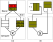
\includegraphics[width=0.4\columnwidth]{figs/deadlock_figs.pdf}
  %\caption{Two forms of network deadlock for CGRA dynamic networks. The left shows input buffer starvation, and the right shows a packet taking an ``illegal'' turn through a node.}
  %\label{fig:deadlock}
%\end{figure}
%Furthermore, because a compute node must be able to send its output to read its inputs, dependences may be propagated backwards through the network; this means that dimension order routing alone is insufficient to make progress and separate virtual networks must be used.
%\subsection{Endpoint Buffer Deadlock}
%This is a type of protocol deadlock that results from head-of-line blocking and finite buffer sizes at node inputs, as shown in Figure~\ref{fig:deadlock}(a).
%Consider two streams, A and B, that traverse the same virtual channel but are destined for different input buffers at the same destination node.
%If A fills up its input buffer, and B's input buffer is empty, the node cannot make progress.
%Simultaneously, if a flit from stream A is at the head of the shared virtual channel, then no flits from stream B will be able to pass it.
%
%At the final hop of the network, this would be trivial to resolve: the final router can use its knowledge of the buffer state of the destination to avoid overloading any single input buffer.
%However, it could be too late to resolve this problem at the final router, because if it blocks the faster flow, and they share a network resource earlier, the slower flow could be head-of-line blocked earlier in the network.
%\subsection{Through-Node Deadlock}
%Because nodes do not have infinite buffers, the deadlock graph for a network no longer begins and ends at the routes---it must be extended with information about the program nodes \cite{hansson2007avoiding}.
%%This means that traditional deadlock avoidance techniques, such as dimension-order routing, are \emph{not sufficient} to prevent deadlock in these networks.
%An example of how this can cause deadlock in a y-first dimension-order routed network is shown in Figure~\ref{fig:deadlock}(b).
%This type of deadlock can also combine with endpoint deadlock, in addition to traditional network deadlock.
%Because nodes propagate holds/waits dependences, any indirect input to the final node is capable of creating an endpoint buffer deadlock at the final node with any other indirect input, anywhere in the network.
%When different branches of the tree are fed by different DRAM accesses, one will almost certainly run faster and inevitably lead to this deadlock condition.
%Practically, this means that no two logical paths may be allowed to conflict at \emph{any} point in the network; to meet this guarantee, buffer allocation is performed to ensure that all logical paths traversing the same physical link are placed into separate virtual channels.
%Because there are only a finite number of VCs at each router, this is another network constraint to optimize: routes are penalized for exceeding the maximum, which leads to them being moved and a better solution being found.

\subsection{Runtime Analysis for Heuristic Generation} \label{sec:heuristic}

In Spatial, the user can annotate runtime-variable input values to assist compiler analysis.  
We use these programmer annotations to compute the expected number of iterations each basic block
will execute. 
The execution count on basic block can future used to derive the packet count produced
by these basic block.
If the control is data-dependent, the user can annotate the data-dependent loop range, or the
fraction for how frequently the branches evaluating to true.
These heuristic guides can help placer to evenly spread out the traffic.
However, we do not require exact annotations for efficient placement---a rough estimate of 
data size is sufficient for the placer to determine the relative importance of links.

Using the estimated packet counts, the placer prioritizes highly used links for allocation to the static network and leaves infrequently used links on the dynamic network. 
When no annotation is provided, or loop bounds cannot be constant-propagated, the compiler estimates
loop iteration counts based on the nesting depth: packets generated by the innermost loops are 
the more likely to be frequent.
This heuristic provides a reasonable estimate of links' priorities for routing purposes.

\todo{Elaborate on how to perform the analysis especially for streaming program}

\section{Debugging and Instrumentation Support (WIP)}
\subsubsection{Deadlock in Streaming Reconfigurable Architecture}

\subsubsection{Debugging Support and Performance Instrumentation}

\section{Evaluation} \label{sec:eval}

In this section, we evaluate the scalability of designs generated by \name.
We also compare the absolute performance of a Plasticine chip compiled with \name against a Tesla V100 GPU 
for a mix of deep learning, sorting, graph processing, and streaming applications.

For our baseline implementation on GPU, we use frameworks and libraries whenever possible, such as TensorFlow compiled
with cuDNN library for deep learning and Gunrock library~\cite{gunrock} for graph applications.
When no library is available, we implement and hand optimize the CUDA implementation.

To better match the V100's peak FLOPS, 
we increase the Plasticine array from a $16\times8$ to a $20\times20$ configuration.
The area footprint of this configuration is \SI{352}{mm^2} at 28nm, which is still well below the 
\SI{815}{mm^2} at 12nm for V100.
We could not match in die area, as the speed of our cycle-accurate simulator limits our selection of Plasticine size.
To match in GPU's off-chip bandwidth, 
we integrate an open-source DRAM simulator--Ramulator~\cite{ramulator}--with our
cycle-accurate simulator to model the HBM2 technology, providing a \SI{1}{TB/s} off-chip bandwidth.

\begin{figure*}
\centering
\includegraphics[width=1\textwidth]{/Users/yaqiz/pldi20/paper/figures/par_thesis.pdf}
\caption[Scalability Evaluation]{
  Scalability Evaluation. 
  Benchmarks include multi-layer perceptron (mlp), BlackScholes (bs), random forests (rf), page rank
  (pr), and long short-term memory recurrent neural network~\cite{hochreiter1997long}.
  The first four charts show the scaling of
  (a) throughput, 
  (b) resource usage, 
  (c) runtime activation rate of PUs on the critical path of the compute pipeline, 
  and (d) achieved HBM bandwidth, as the program gets parallelized.
  (e) shows the combined design space of compiler optimizations and parallelization factors on a
  throughput-resource curve. 
  The Pareto frontier presents the throughput improvement with an increasing resource by drawing the y-axis in (a) as a function of the y-axis in (b).
}
\label{fig:par}
\end{figure*}

\subsection{Scalability}
\Cref{fig:par} shows how performance and on-chip resources vary as the application gets parallelized in
(a-d). 
For each parallelization factor, we evaluate a combination of various compiler flags, presenting the
best configurations in (a-d).
Starting with a non-parallelized and fully pipelined design, 
we incrementally parallelize the critical stages of the pipeline with the lowest throughput.
For \textbf{mlp}, for example, this corresponds to the dense layer with the most operations.
For DRAM-bound applications, like \textbf{rf}, we increase the number of parallel DRAM streams.
\Cref{fig:par} (a) shows an almost perfect performance scaling for most compute-bound apps, including
\textbf{mlp}, \textbf{bs}, and \textbf{lstm}.
The DRAM-bound applications, i.e. \textbf{rf} and \textbf{pr}, achieve a perfect scaling until
saturating in DRAM bandwidth, as shown in (c).

As we discussed in the MLP case study in \Cref{fig:mlp} and shown in (b), the resource does not
monotonically increase with parallelization factor due to optimizations discussed in \Cref{sec:opt},
which explains the dip in the \textbf{mlp} curve in (a). 
With further investigation, we found the best set of compiler flags that gives the perfect scaling 
did not fit in resource at parallelization factor of 240; hence, a flag combination using less
resource with less performance is presented. 
A design with the optimum flags consumes less resource at a higher parallelization factor at 256, 
as a power of two factor enables more optimizations, which continues the scaling.

The resource in (b) increases slowly with a small parallelization factor. This is because initially,
as the pipeline is highly imbalanced, \name only needs to parallelize a small portion of the
entire pipeline to improve overall throughput. As the pipeline gets balanced, \name must parallelize
all stages in the pipeline to further enhance throughput. Larger parallelization factor also comes
with the expensive crossbar connection from memory partitioning discussed in~\Cref{sec:memsplit}.

\Cref{fig:par} (c) shows the activation rate of the critical pipeline stages at runtime.
A close to 100\% activation rate at close to 100\% resources (400 PUs) suggests that 
\name introduces minimum synchronization overhead and is truly scalable.
The decreasing in the activation rate in \textbf{lstm} is due to increasing initiation interval
(II)~\cite{II} with large parallelization.
The recurrent neural network contains an inherent loop-carried dependency (LCD) in the algorithm. 
As we parallelize a stage with a reduction within the cycle of LCD, the latency of the reduction tree
also increases, resulting in a larger II that slows down the pipeline runtime.

\Cref{fig:par} (e) shows the full design space of performance-resource trade-off with
different parallelization factors and compiler optimizations.
We can see that compiler optimizations play an important role in improving performance or
reducing resource that pushes the Pareto leftwards and upwards.

%\begin{figure*}
%\centering
%\includegraphics[width=1\textwidth]{/Users/yaqiz/pldi20/paper/figures/par.pdf}
%\caption[Performance comparison with V100 GPU]{
%}
%\label{fig:par}
%\end{figure*}

\subsection{Comparison with a GPU}

\Cref{tab:gpu-comparison} shows the throughput and latency comparison with a Tesla V100 GPU.
\Cref{fig:speedup} presents the speedup with Plasticine.
In additional to raw measurements from simulation, we also present an area-normalized throughput
taking into account of the technology difference between Plasticine and V100 
for SqueezeNet 1.0~\cite{squeezenet} and LSTM~\cite{lstm}; 
these applications are compute-bound and hence their throughputs are proportional to available 
on-chip resources.

\begin{figure}
\begin{table}[H]
  \centering
    \footnotesize
    \begin{tabular}{lcccccc}
    \toprule
      \multirow{2}{*}{\textbf{Benchmark}} &
      \multirow{2}{*}{\makecell[c]{\bf Throughout\\\bf Unit}} &
      \multirow{2}{*}{\makecell[c]{\bf GPU\\\bf Compiler}} & \multicolumn{2}{c}{\textbf{Latency} (ms)} &
      \multicolumn{2}{c}{\textbf{Throughput} (Unit/s)} \\
                                & & & \name & GPU & \name & GPU     \\
      \midrule
        SqueezeNet (batch-1) & {\em kFrames}   & TF+cuDNN & 49.13  & 70.10  & 0.12 (1.1) & 0.4   \\ \addlinespace
        LSTM (batch-32)      & {\em kSamples}  & TF+cuDNN & 3.61   & 6.81   & 8.8 (79.2) & 4.7   \\ \addlinespace
        PageRank             & {\em MEdges}    & Gunrock & 128.27 & 829.39 & 49         & 7.5   \\ \addlinespace
        BlackScholes         & {\em GOptions}  & CUDA & 0.09   & 0.10   & 88.88      & 80.02 \\ \addlinespace
        Random Forest        & {\em MSamples}  & CUDA & 0.10   & 0.32   & 1.04       & 0.32  \\ \addlinespace
        Merge Sort           & {\em GElements} & CUDA & 0.63   & 2.14   & 6.65       & 1.96  \\
      \bottomrule
    \end{tabular}
  \caption{Performance comparison of Plasticine with Tesla's V100 GPU (Normalized throughput to transistor count in parentheses).}
  \label{tab:gpu-comparison}
\end{table}
\begin{figure}[H]
\centering
\includegraphics[width=1\textwidth]{figs/slide_gpu.pdf}
\caption[Performance comparison with a Tesla V100 GPU]{
  Plasticine's latency and throughout improvement over V100 GPU.
  The evaluated Plasticine architecture has area footprint of 352$mm^2$ at 28nm.
  V100 GPU has area footprint of 815$mm^2$ at 12nm.
  Both platforms have the same off-chip bandwidth at 1TB/s with HBM technology.
  Yellow and blue bars show the raw measured speedup in throughput and latency, respectively.
  To account for the resource discrepancy, the pink bar shows the normalized throughput
  for compute-bound application--SqueezeNet and LSTM, which scales performance with additionally
  on-chip resources.
}
\label{fig:speedup}
\end{figure}
\end{figure}

\paragraph{Neural Networks} 
After normalized in resource, Plasticine shows a 2.75x and 16.85x speedup in throughput for the
compute-bound applications--SqueezeNet and LSTM.
These applications benefit from the flexible degrees of parallelism \name{} exploits. 
In addition to streaming pipelining across network layers, \name can also parallelize on the
input and output channels/dimensions of a single convolution/dense layer in SqueezeNet/LSTM.
In contrast, GPU needs to accumulate a large batch size to fully utilize the parallel threads.
SqueezeNet also has a highly imbalanced pipeline, with 2x more computation in certain layers than
the others.
Exploiting pipeline parallelism allows Plasticine to distribute the most resources to the program
phase with the most operations.
GPU executes these layers in time and parallelizes them equally; 
layers with fewer operations are likely to underutilize the chip.

\paragraph{BlackScholes} 
Both Plasticine and V100 can saturate HBM2 bandwidth for BlackScholes.

\paragraph{PageRank} 
PageRank implemented in \name achieves a 6.5x latency speedup and throughput improvement comparing
to Gunrock \cite{gunrock} on the denaulay\_n20 \cite{delaunayn20} dataset. 
Due to the SIMT restriction in GPU, Gunrock only explore edge frontier parallelism, 
which underutilizes the hardware when the graph is sparse.
In contrast, \name{} parallelizes both the edge and node processing across multiple DRAM streams.
\name can exploit arbitrary levels of hierarchical parallelism on non-perfectly nested loops,
resulting in a perfect scaling of PageRank shown in~\Cref{fig:par} (a).

\paragraph{RandomForest} We created a synthesized tree model that contains 8 estimator trees and 128 splits per estimator. 
Implementation with \name{} on Plasticine shows 3.2x speedup comparing to the implementation in CUDA on V100. 
Similarly to BlackScholes, RandomForest contains a massive basic block with multiple tree
structures in the dataflow graph corresponding to the estimators.
GPU executes this basic block in time. 
As a result, the irregular memory access from the graph structure causes bad memory performance in V100.
In contrast, \name{} maps the entire dataflow graph spatially across PUs, vectorizing across a batch of 16 samples.
The entire basic block is streaming pipelined at full throughout without any memory access.

\paragraph{MergeSort} 
The merge tree implementation on Plasticine uses a multi-way merging tree to merge the sorted
partitions stored in the off-chip memory iteratively.
This implementation saturates off-chip bandwidth by parallelizing on multiple DRAM streams within
each iteration.
We compared merge sort and radix sort on GPU and took the radix sort with a faster runtime.
Overall, sorting on Plasticine implemented with \name provides 3.4x latency speedup and throughput
improvement against the GPU.


